\documentclass[main.tex]{subfiles}
 
\begin{document}
In this final chapter, we discuss the results of applying our theory to the SciGRID dataset. We would like to reiterate that this data is aggregated from different sources, most of which are \emph{not} physical measurements, but `educated guesses'.

With this in mind, we proceed with our analysis, not necessarily with the goal of providing accurate operational advice for German grid operators, but to demonstrate that the model can be applied to real-world transmission networks. By studying a representative dataset, we can study the strengths and weaknesses of the model. Finally, we hope that this model will provide \emph{qualitative insight} into the complex behaviour of grid failures, not specific to this dataset.

\towrite{Iets zeggen over \emph{hoe} (on)nauwkeurig we zijn. Bijvoorbeeld: zorgen kleine veranderingen in de dataset voor grote veranderingen in resultaten?}

\section{SciGRID data}
The SciGRID dataset needs to be translated into the language of our model. It contains more information than we need, and it is not yet in the desired format. 

\subsection{Structure}
\emph{(A more detailed analysis of dataset properties is available on the GitHub repository.)}

Before any processing, we find that the SciGRID network (obtained from \texttt{PyPSA} example code, the exact dataset used by \cite{Nesti2018emergentfailures}) contains 585 buses, 1423 generators (of all sources) and 489 loads. It also contains 38 storage units (all are pumped hydroelectric), but these were excluded from our analysis.\footnote{More specifically, they were used in solving the OPF problem, but their initial charge was set to zero.} There are 852 transmission lines in the dataset, at possible voltage levels $220 \, \si{\kilo\volt}$ and $380 \, \si{\kilo\volt}$, and there are 96 transformers (between these two voltages). Transmission lines have per-kilometre estimates for admittance, from which the total admittance can be deduced.

\subsubsection{Voltages}
In our model, we \emph{normalise} the grid voltage. To do so, we multiply all line admittances by the \emph{square} of their operating voltages, after which all voltages can be assumed to be $1$, and a unit of current is proportional to a unit of transmitted power. Of the 585 buses, 192 are part of one of the 96 \emph{voltage pairs}: these are two buses at the same location, with the same name (except for the voltage suffix), connected via a transformer. By merging these pairs, we find 489 geographically unique buses, at normalised voltage. From now on, we will refer to these (possibly merged) buses as the buses of the network: $n=489$, $\mathcal{N} = \range{489}$.

\subsubsection{Loads}
There is exactly 1 load connected to each bus. In reality, there are of course thousands of loads connected to a bus, but the load in the dataset is the \emph{aggregated} load at that bus. We have hourly time series (\ie amount of $\si{\mega\watt}$ being consumed) for each node in the year 2011, which only includes active power consumption.

\subsubsection{Generators}
Generators are connected to the geographically closest bus, and there is at most one generator per bus of each type.\footnote{In order of installed capacity: \emph{Wind Onshore} ($37\,\si{\giga\watt}$), \emph{Solar} ($37\,\si{\giga\watt}$), \emph{Hard Coal} ($25\,\si{\giga\watt}$), \emph{Gas} ($24\,\si{\giga\watt}$), \emph{Brown Coal} ($21\,\si{\giga\watt}$), \emph{Nuclear} ($12\,\si{\giga\watt}$), \emph{Run of River} ($4\,\si{\giga\watt}$), \emph{Other} ($3\,\si{\giga\watt}$), \emph{Wind Offshore} ($3\,\si{\giga\watt}$), \emph{Oil} ($2.7\,\si{\giga\watt}$), \emph{Waste} ($1.6\,\si{\giga\watt}$), \emph{Storage Hydro} ($1.4\,\si{\giga\watt}$), \emph{Multiple} ($0.15\,\si{\giga\watt}$) and \emph{Geothermal} ($32\,\si{\mega\watt}$).} This means that generation is \emph{aggregated}: multiple generators of the same type are combined into one. There are 489 solar generators, 488 onshore wind generators and 5 offshore wind generators. Offshore wind generators are connected to buses at the north coast of Germany. This means that every bus houses stochastic generation. Their geographic distribution is shown in Figure~\ref{fig:solarwind}.

\subsubsection{Lines}
Line voltages and admittances are normalised as described above. For each line, we have the names of the two original buses that it connects, which can easily be converted to the new bus collection.

During the study of cascading failures, we found that the network contains \emph{parallel lines}: lines that connect the same pairs of buses. In some cases, there are up to four different lines that are all parallel. When examining these cases on OpenStreetMap, we find that there are indeed parallel lines in the physical network. This is reflected by the \emph{lengths} of parallel lines, as given by SciGRID: these are not the great-circle distances between buses, but rather the distance measured along the line (which makes some turns and bends).

Because our model only holds for \emph{digraphs}, which cannot have parallel lines, we \emph{combine} parallel lines, by summing their (voltage normalised) admittances, and summing their thresholds.\footnote{The results regarding the kernel of $\FRT$, and the Optimised method for analysis cascading failures, break down without this property.} \cite{Nesti2018emergentfailures} do not mention this anomaly, and use the original set of lines. For comparison, we computed some results for both versions of the network, and found the results to be somewhat similar, in general. Because we did not consider the case of parallel lines in our model, combining parallel lines in the dataset seems like the \emph{correct} choice.

Of the 852 original lines, there are 705 unique links between original buses before normalising voltages, and there are 695 unique links between buses. There are never two parallel lines with opposite orientation. These 695 lines were used in our model, and will be referred to as simply the \emph{lines} of the network: $m = 695$.

\subsection{State}
Our dataset contains hourly values for load and stochastic (wind and solar) generation for the year 2011. Deterministic generation is estimated using the OPF algorithm, as implemented by \texttt{PyPSA} \citep{PyPSA}, a Python package designed for this purpose. Following common practice, we first multiply all line thresholds by a \define{contingency factor}: $0.70$. This forces the optimisation process to leave a safety margin at every line, and also accounts for the error of using the DC approximation. Figure~\ref{fig:nominalflowandinjection} shows the resulting injection at 1 January 2011 at 11:00. Line currents can then be computed using the LPF.

\begin{figure}[ht]
    \centering
    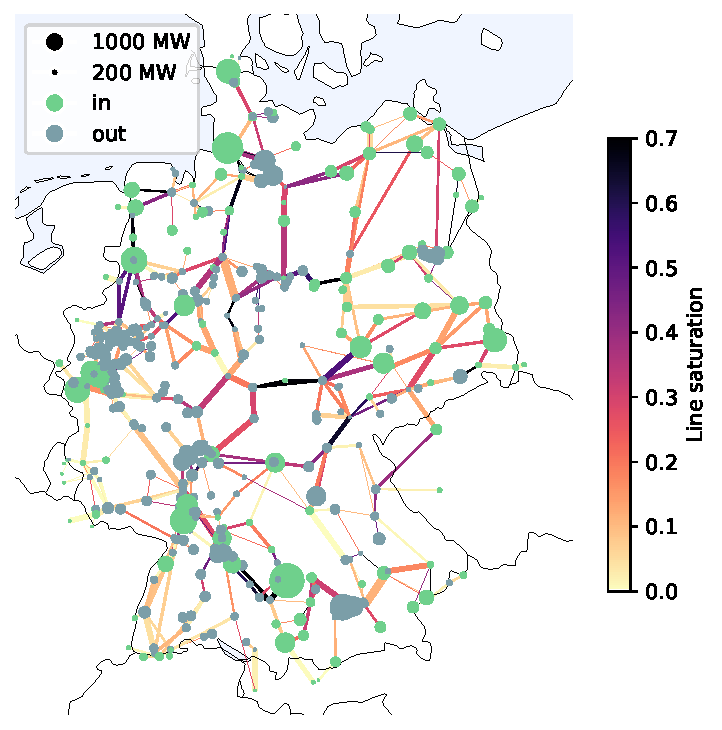
\includegraphics[width=.6\textwidth]{img/nominal_flow_and_injection.pdf}
    \caption{
    \label{fig:nominalflowandinjection}Nominal line flow during 11:00-12:00, as fraction of line capacity. Node size represents net power injection. When generation exceeds load, the injection is positive (green), otherwise negative (greyish blue). \emph{Compare with Figure 1a of \cite{Nesti2018emergentfailures}.}}
\end{figure}

\section{Bus covariance}
As discussed in Section~\ref{sec:persistentforecast}, we estimate the bus covariance matrix from historical errors in our forecast. We find \emph{high} covariances among nodes, which we expected from our preliminary analysis. Because renewable generation data is extrapolated directly from (coarse) weather data, the generation series of nearby buses are almost identical. 

The covariance of buses, calculated using the difference series, is visualised in Figure \ref{fig:buscov}. 
\begin{figure}[ht]
    \centering
    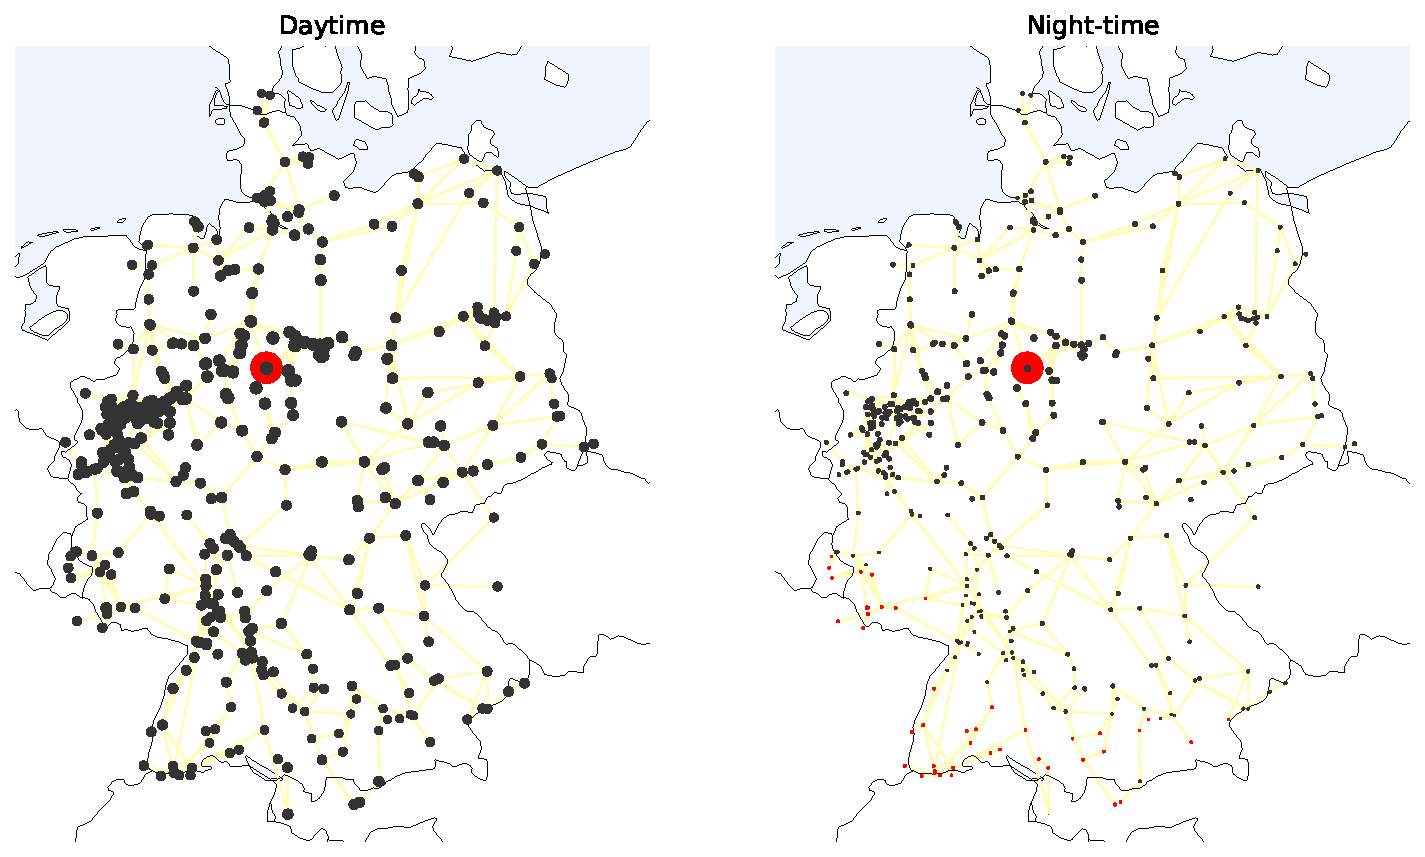
\includegraphics[width=\textwidth]{img/bus_correlation_123_fullcov_day_and_night.pdf}
    \caption{
    \label{fig:buscov}Covariance of all buses, relative to the circled bus. Normalised using installed renewable capacity.}
\end{figure}

\section{Line covariance}
By incorporating bus covariances in our model (which result from correlated weather), we hope to find new structure in the line covariances. 
To assess the effect of estimating bus covariances, we compare three possible bus covariance matrices:
\begin{enumerate}
	\item \emph{The identity matrix}: all bus injections are independently Gaussian distributed with the same variance. (They are almost IID, but their means differ.)
	\item \emph{The diagonal of estimated variances}: all bus injections are independently Gaussian distributed, but their variances and means differ.
	\item \emph{The estimated covariances}: the vector of bus injections is (multivariate) Gaussian distributed. All bus injections are, in general, dependent on each other, and their variances and means differ.
\end{enumerate}

It is well known that local changes to the grid structure have long-range effects. For example, \cite{Witthaut2013} showed that \emph{adding} a new line to a heavily congested, but stable network can cause the failure of another line, possibly far away from the added line.\footnote{The counter-intuitive fact that adding a line, or increasing the impedance of existing lines, can make a network \emph{more} congested, is known as \define{Braess' Paradox}. Similarly, some line failures can be \emph{prevented} by switching off other lines in the network. See Figure~\ref{fig:braess} for a minimal example.} This is reflected in our model by the fact that line currents have non-zero covariance, even when bus injections are independently distributed. (In this case, $\mat{\Sigma}_{\mat{f}} = \mat{F}\mat{I}\mat{F}^* = \mat{F}\mat{F}^*$, which is generally not a diagonal matrix.) Figure~\ref{fig:linecov1} and Figure~\ref{fig:linecov2} show the covariances of all lines, relative to a chosen line. We see that covariance is generally high for lines that are close, but there are some clear exceptions. There seems to be a general trend that lines are highly (positively or negatively) correlated when they are close, and \emph{oriented in the same direction} (\eg East-West) as the chosen line.

\begin{figure}[ht]
\centering
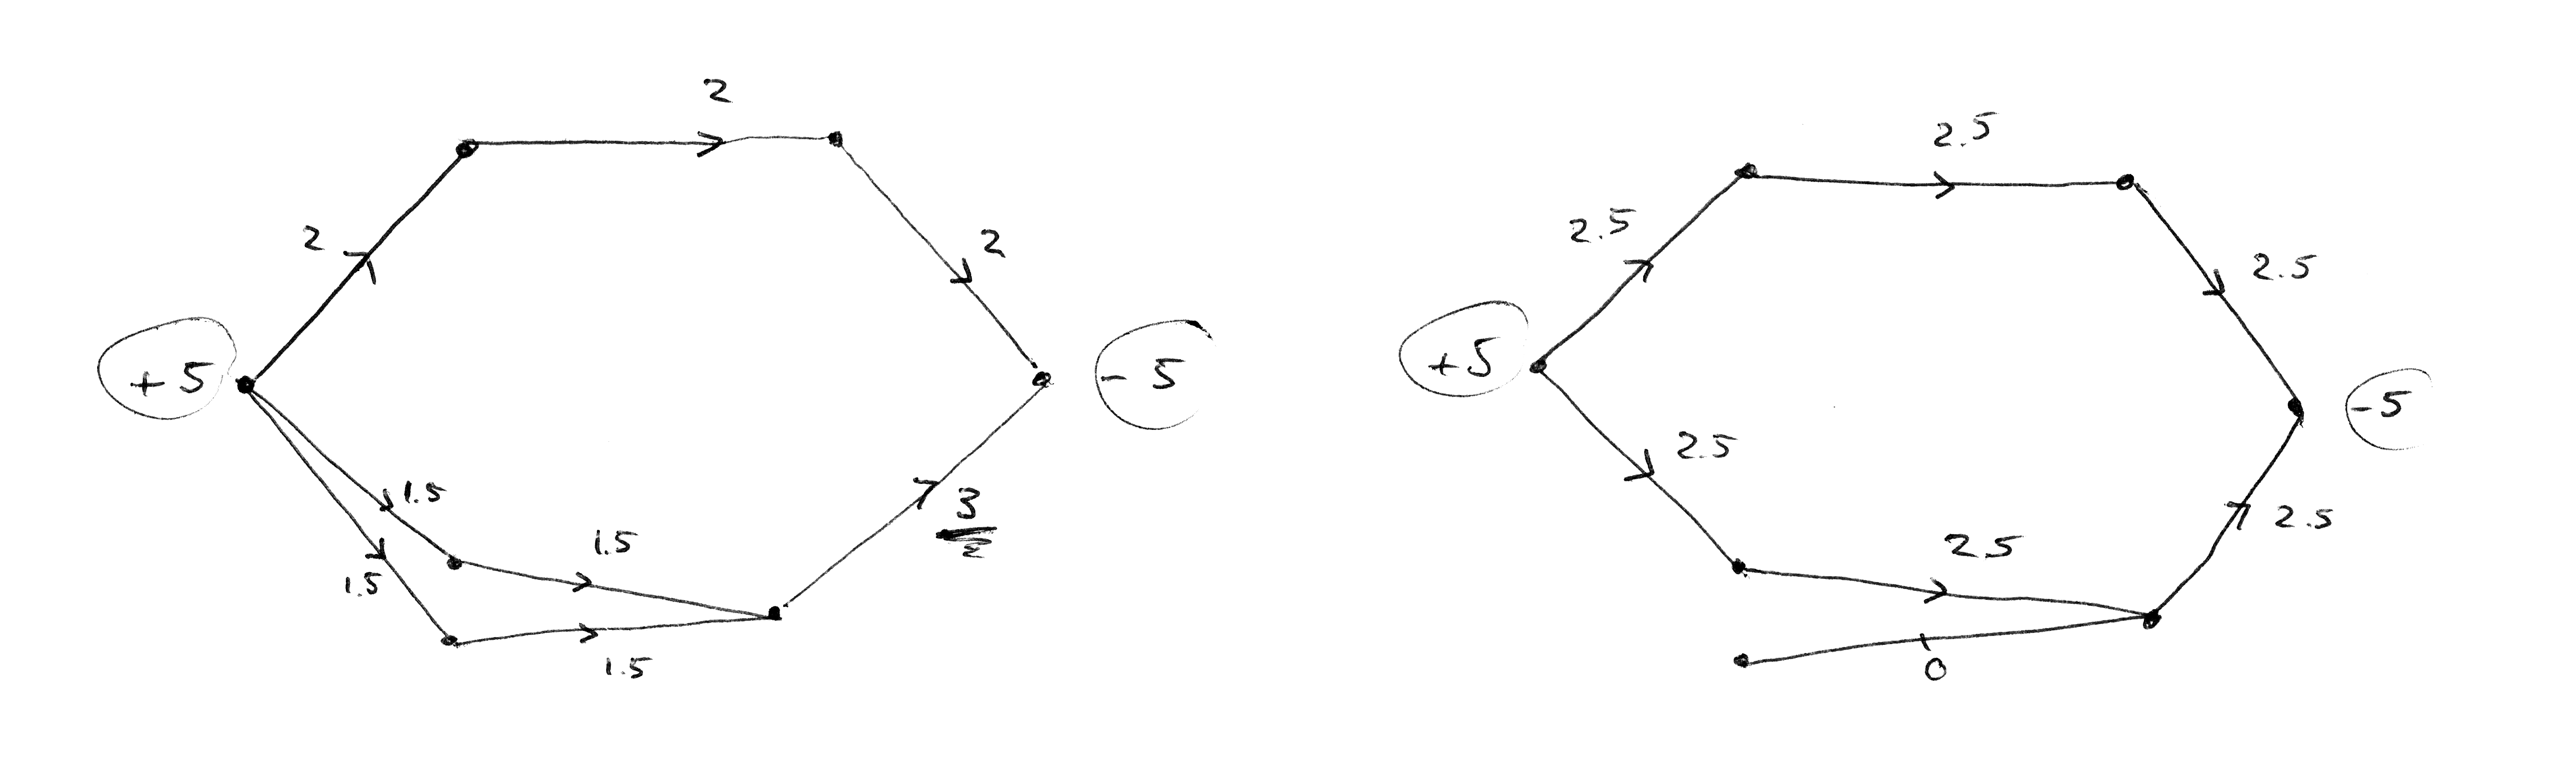
\includegraphics[width=\textwidth]{img/braesstekening.png}
\caption{\label{fig:braess} PLACEHOLDER: An example of Braess' Paradox. A network transporting $5$ units of power from left to right; all lines have the same admittance, and threshold $3$. On the left, one line (lower right) is overloaded. When this line fails, all power will travel through the upper branch, causing it to overload as well, leaving the network disconnected. If instead, the \emph{lower left} line is switched off, the flow of power will be more evenly distributed, and no line will overload. Of course, this example also illustrates how adding a line could lead to overloads.}
\end{figure}

\begin{figure}[ht]
\begin{subfigure}{\textwidth}
    \centering
    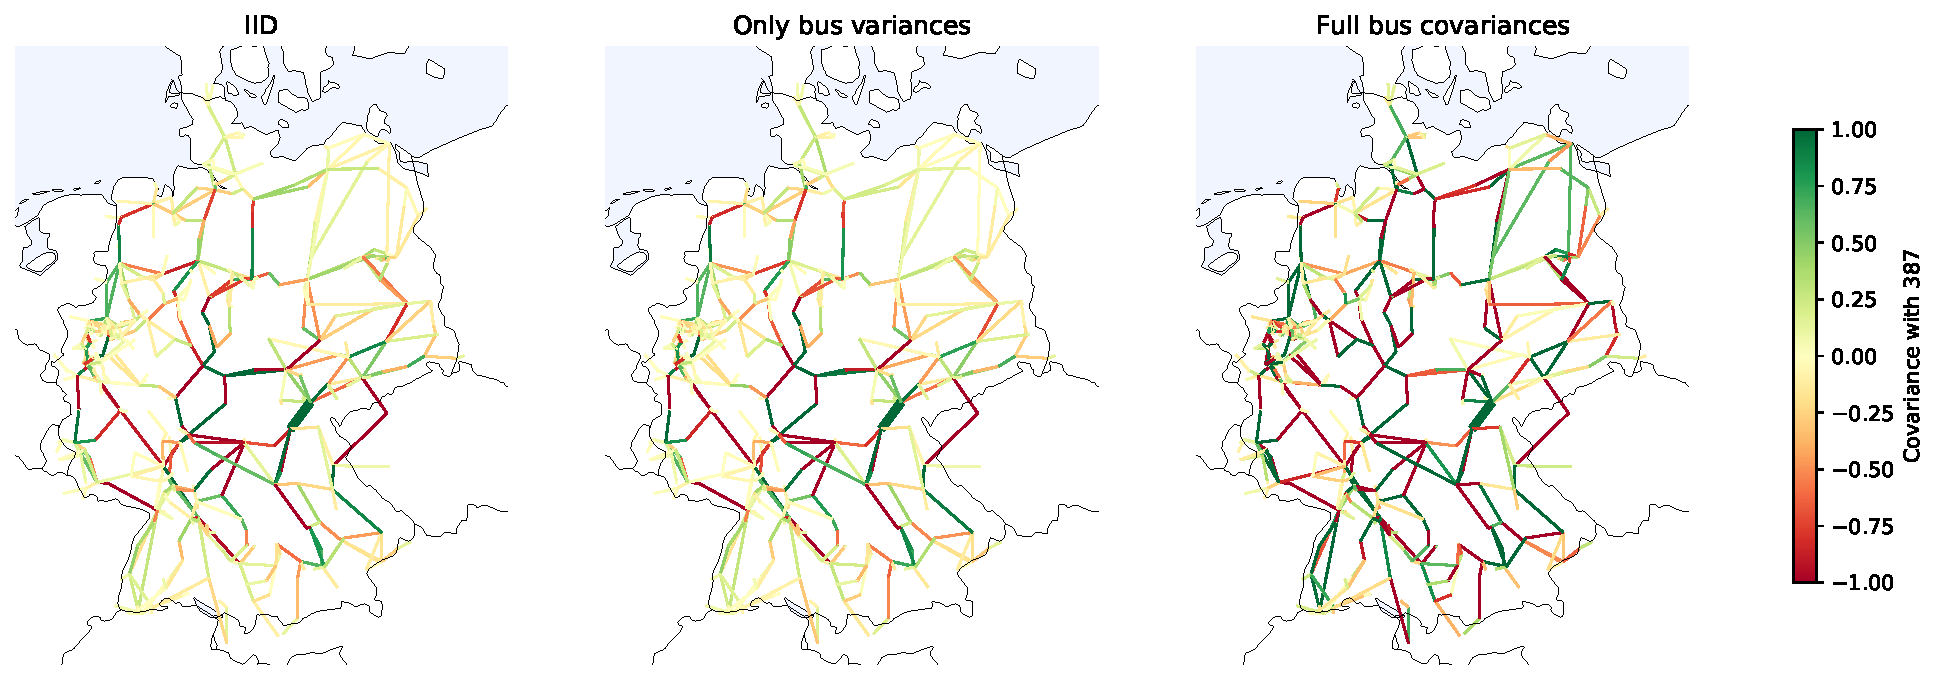
\includegraphics[width=\textwidth]{img/flow_correlation_387_iid_and_justvar_and_fullcov.pdf}
    \caption{Covariances relative to line 387.}\label{fig:linecov1}
\end{subfigure}
\begin{subfigure}{\textwidth}
    \centering
    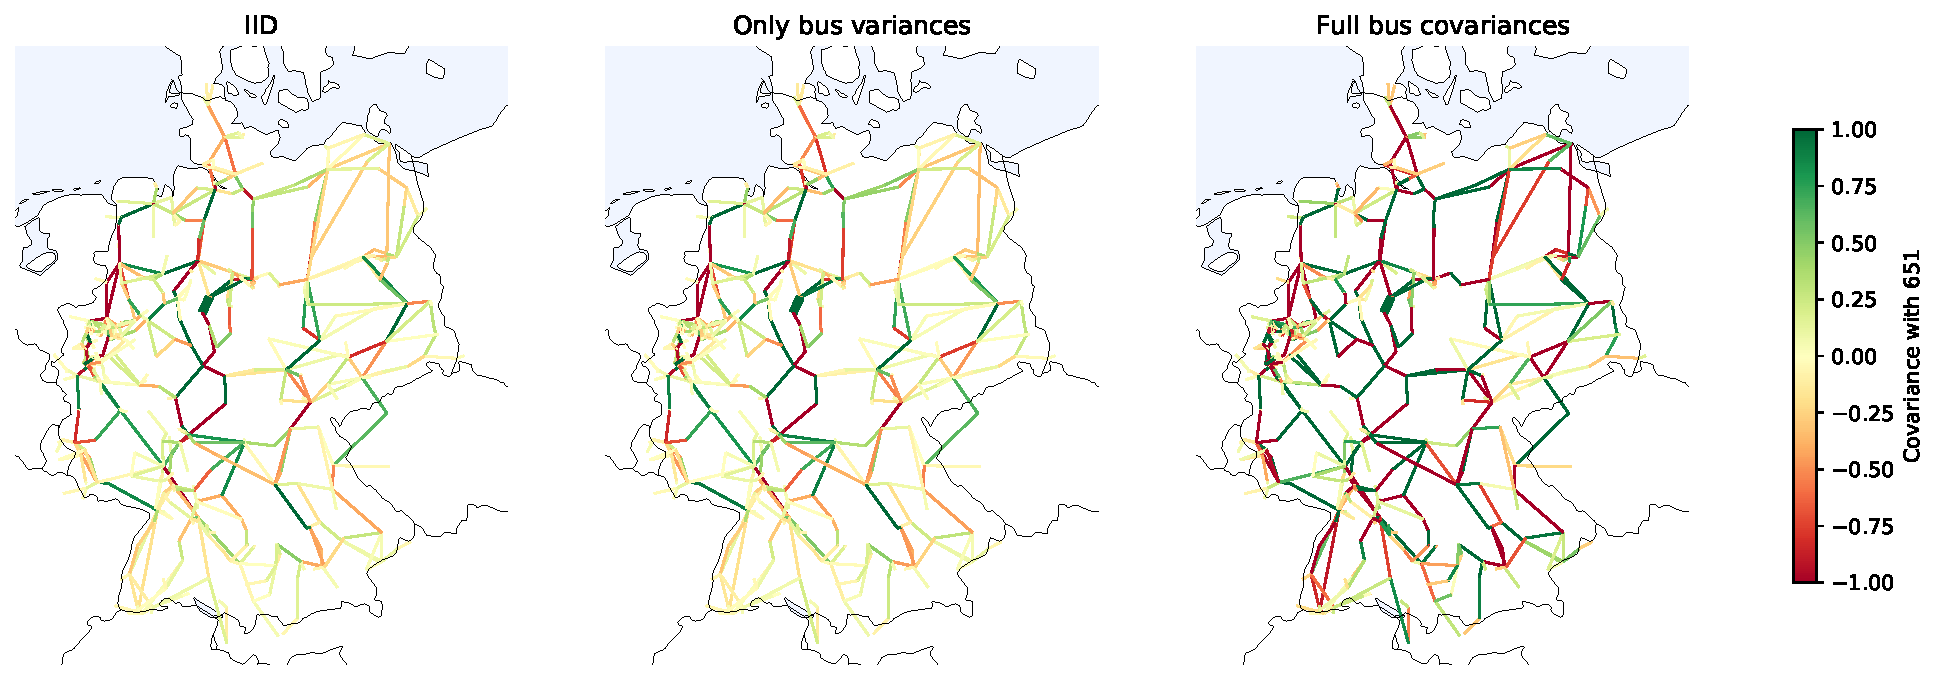
\includegraphics[width=\textwidth]{img/flow_correlation_651_iid_and_justvar_and_fullcov.pdf}
    \caption{Covariances relative to line 651.}\label{fig:linecov2}
\end{subfigure}
    \caption{Covariance of all lines, relative to the enlarged line. Normalised using installed renewable capacity. Signs (red or green) can be chosen arbitrarily. Absolute covariance is therefore proportional to color \emph{saturation}.}
\end{figure}

The covariance of a random pair of lines is relatively high, when their physical separation (measured either in kilometres or in graph distance) is low. Because weather is correlated, even at high distance, using the bus full covariance might result in higher covariances between lines with high separation. (This was concluded by \cite{Nesti2018emergentfailures}.) 

Using a different bus covariance matrix will likely result in a overall increase or decrease of line covariances. Note, however, that the line covariance matrix is scaled by an arbitrary factor $\epsilon$, so any overall change in covariance has no significance in the model. 

This makes it difficult to compare the three bus covariance matrices, as any absolute difference in line covariance should be ignored. Instead, we will examine the covariance of two lines, \emph{relative to their own variances}. This way, the effect of any absolute, proportional increase in covariance is avoided. First, let us choose a number of lines, and examine the covariances of all other lines with the chosen line, relative to its variance. 

In particular, we are interested in the decay of covariance over distance. \cite{Jung2016} studied the decay of the Line Addition Distribution Factor (difference in flow after adding a line) over distance, also using the SciGRID network. This is not the same as covariance, of course, but both are measures of the \emph{global effect} of local changes in flow. They first determined the largest 2-connected component of the network, and removed all other lines from the model. In the remaining network, they studied the 880 possible additions of short new lines, and found a general \emph{exponential} decay of change in currents as a function of graph distance.

To study the decay of covariance, we collect the geographical separation and covariance (resulting from the three possible bus covariance matrices) of $10^5$ random pairs of lines in the network. Because of power flow physics, these covariances are highly spread out. However, when averaging the covariances in groups of $25 \, \si{\kilo\metre}$ (Figure~\ref{fig:linecovdecay}), we find are able to see the differences in decay. 

\begin{figure}
\centering
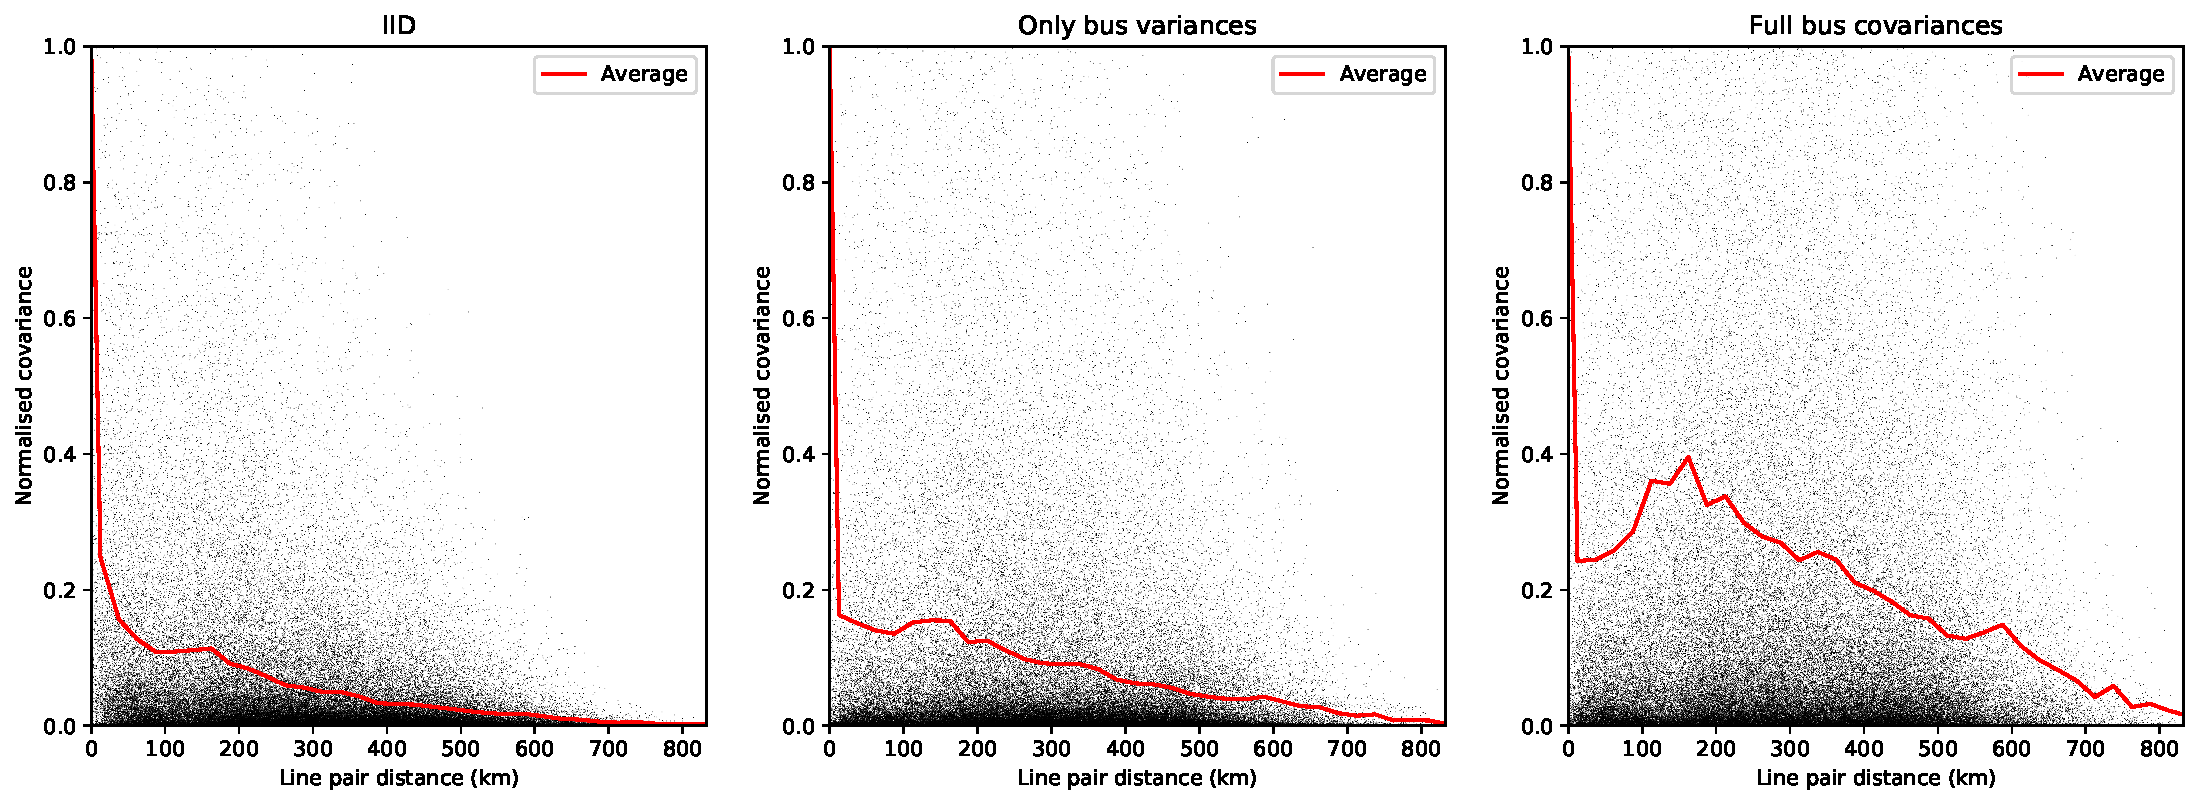
\includegraphics[width=\textwidth]{img/covariance_linepairs_with_average.pdf}
\caption{\label{fig:linecovdecay} For $10^5$ random pairs of lines, the covariance and distance (between line centres) is shown, for three possible bus covariance matrices. The averages (over $25 \, \si{\kilo\metre}$) show that correlated buses increase long-range correlations in line flows. Covariances are normalised using average line variance.}
\end{figure}

\todo{Maar als je normaliseert op variantie?}
\towrite{Compare three bus covariance }
By doing so, we find an important result. When we model bus injections to be uncorrelated (first two graphs in Figure~\ref{fig:linecovdecay}), we find \emph{some} correlation in line flows, which are due to power flow physics.\footnote{As an example, consider the $n$-loop network. Here, two neighbouring lines are highly correlated, since they always transmit roughly the same amount of power. (The difference is the amount of power injected at their common node.)} On average, these correlations decrease as the distance between two lines increases, as shown by the red line.\footnote{We might expect this decay to be \emph{exponential} (based on the work of \cite{Jung2016}, for example), but this is not the case.} 
On the other hand, when we include \emph{covariances among bus injections} in our model (last graph in Figure~\ref{fig:linecovdecay}), we find a \emph{relative increase in long-distance correlations of line flows}, compared to the uncorrelated case. This is one of the main results of \cite{Nesti2018emergentfailures}, which they demonstrate only on the $n$-loop network. Figure~\ref{fig:linecovdecay} validates that the result also holds for the SciGRID network.

Curiously, in the range $25\,\si{\kilo\meter}$ - $150\,\si{\kilo\meter}$, the average correlation of line flows \emph{increases} with higher line distances. The reason for this phenomenon is unclear, but one could investigate this further by examining line pairs of these short distances individually.

\begin{figure}
    \centering
    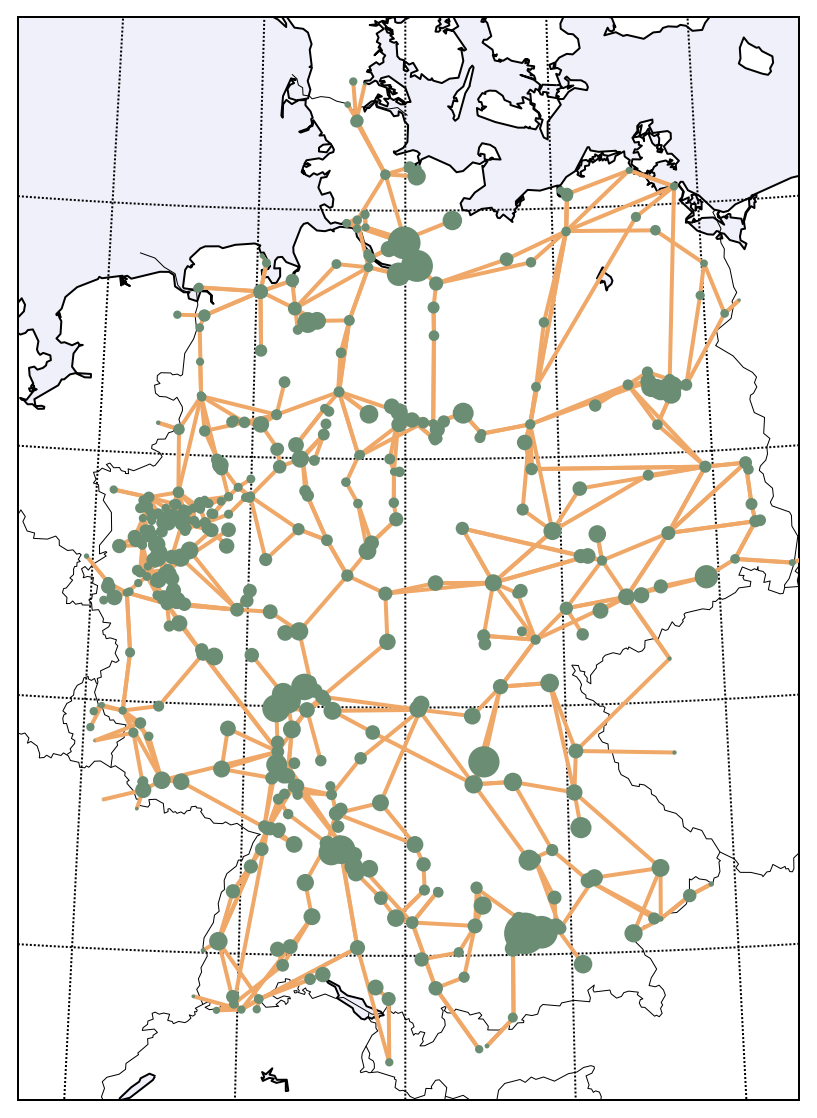
\includegraphics[width=.4\textwidth]{img/load.png}
    \caption{PLACEHOLDER: The load distribution of Germany at ???.}
    \label{fig:loaddistribution}
\end{figure}

\begin{figure}
    \centering
    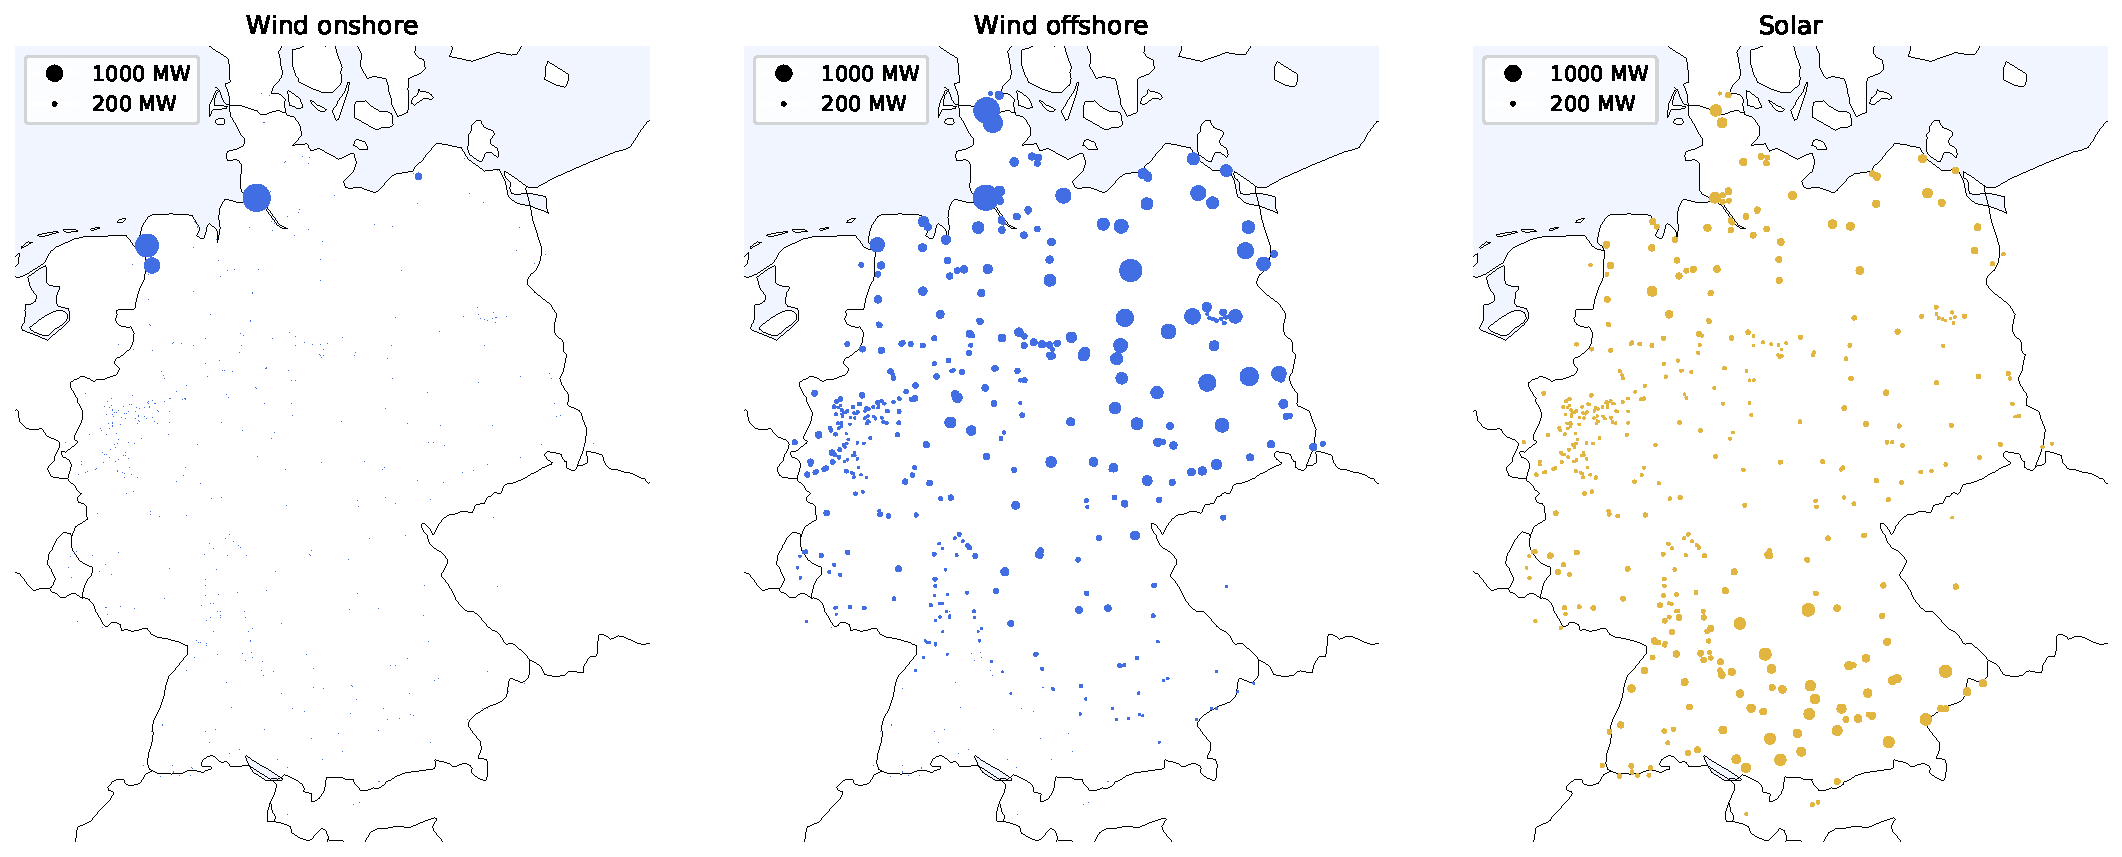
\includegraphics[width=\textwidth]{img/installed_stochastic_capacity.pdf}
    \caption{Installed stochastic capacity per source: wind onshore, wind offshore, solar.}
    \label{fig:solarwind}
\end{figure}


\section{Most vulnerable lines}
Using the nominal injection at 1 January, 11:00, we compute the failure probability of each line. The 30 most vulnerable lines are given in Table~\ref{tab:results} (first two columns) and their positions are given in Figure~\ref{fig:nomflow_stdev_overload}. In the SciGRID dataset, lines are not numbered randomly. Rather, we find that two consecutive line numbers often correspond to two lines that are in close proximity. In the case of lines 651 and 652, for example, the two lines are connected in \emph{series}. As a consequence of power flow physics, their line flows highly correlated.

We identify the same vulnerable lines as \cite{Nesti2018supplemental}, but the ranking is different. This can be attributed to two differences in approach. First, we have combined parallel lines,\footnote{all 30 most vulnerable lines were not part of a parallel combination} which changes the vulnerability order significantly. It is unclear why this changes the result. For comparison, the ranking that we get \emph{without} combining parallels is given in Table~\ref{tab:top20old}, which is more similar that of \cite{Nesti2018supplemental}. The second major difference is the use of a different covariance matrix, although it is reassuring to see that the same lines are identified.

\subsection{Properties of vulnerable lines}
As can clearly be seen in Table~\ref{tab:results}, most lines that are vulnerable to emergent failures are nominally being used at 70\% percent of their capacity. (This is exactly the \emph{contingency factor} used in the LOPF calculation.) This is explained by the low standard deviations of line flows. In fact, when we scale the covariance matrix uniformly by a factor close to zero, this effect is exaggerated.\footnote{This is a \emph{large deviations} result of the normal distribution: if we have $X \, \sim \, \gaussdistr(0, \sigma^2)$, then the marginal distribution of $X \, \mid \, X \geq 1$ becomes increasingly concentrated around $1$ as $\sigma$ tends towards zero. See \eg \cite{Touchette2011}.}

The 10 most vulnerable lines are not significantly long or short. They average $43\,\si{\kilo\meter}$ (SD $30 \,\si{\kilo\meter}$), compared to $36\,\si{\kilo\meter}$ (SD $35 \,\si{\kilo\meter}$) for \emph{all} lines in the network. From Figure~\ref{fig:nomflow_stdev_overload} we can make the interesting observation that vulnerable lines are generally oriented radially towards the \emph{Ruhr}, a density populated area in western Germany.

Vulnerable lines have significantly lower thresholds. On average, the 10 most vulnerable lines can transmit $554 \, \si{\mega\watt}$ (SD $219 \, \si{\mega\watt}$), while the grid-wide average is $1385 \, \si{\mega\watt}$ (SD $1052 \, \si{\mega\watt}$). Indeed, a change in injection has an \emph{absolute} effect on line flows; lines with low thresholds that are operating at the contingency limit (70\%) need only a small amount of additional power to overload.

There is a difference in line \emph{impedance}: $3.9 + 18.9i \, \si{\ohm}$ (SD $3.3 + 12.5i \, \si{\ohm}$) compared to the average of all lines, $2.0 + 12.0i \, \si{\ohm}$ (SD $2.6 + 13.6i \, \si{\ohm}$). This higher reactance means that vulnerable lines have higher \emph{susceptance}, making them more sensitive to changes in node voltages. Grid operators have some control over these values, and lowering the line reactance might make these lines less vulnerable. To study these questions further, we need to also take \emph{reactive power} into account, which we omitted in the DC approximation.

\begin{figure}
    \centering
    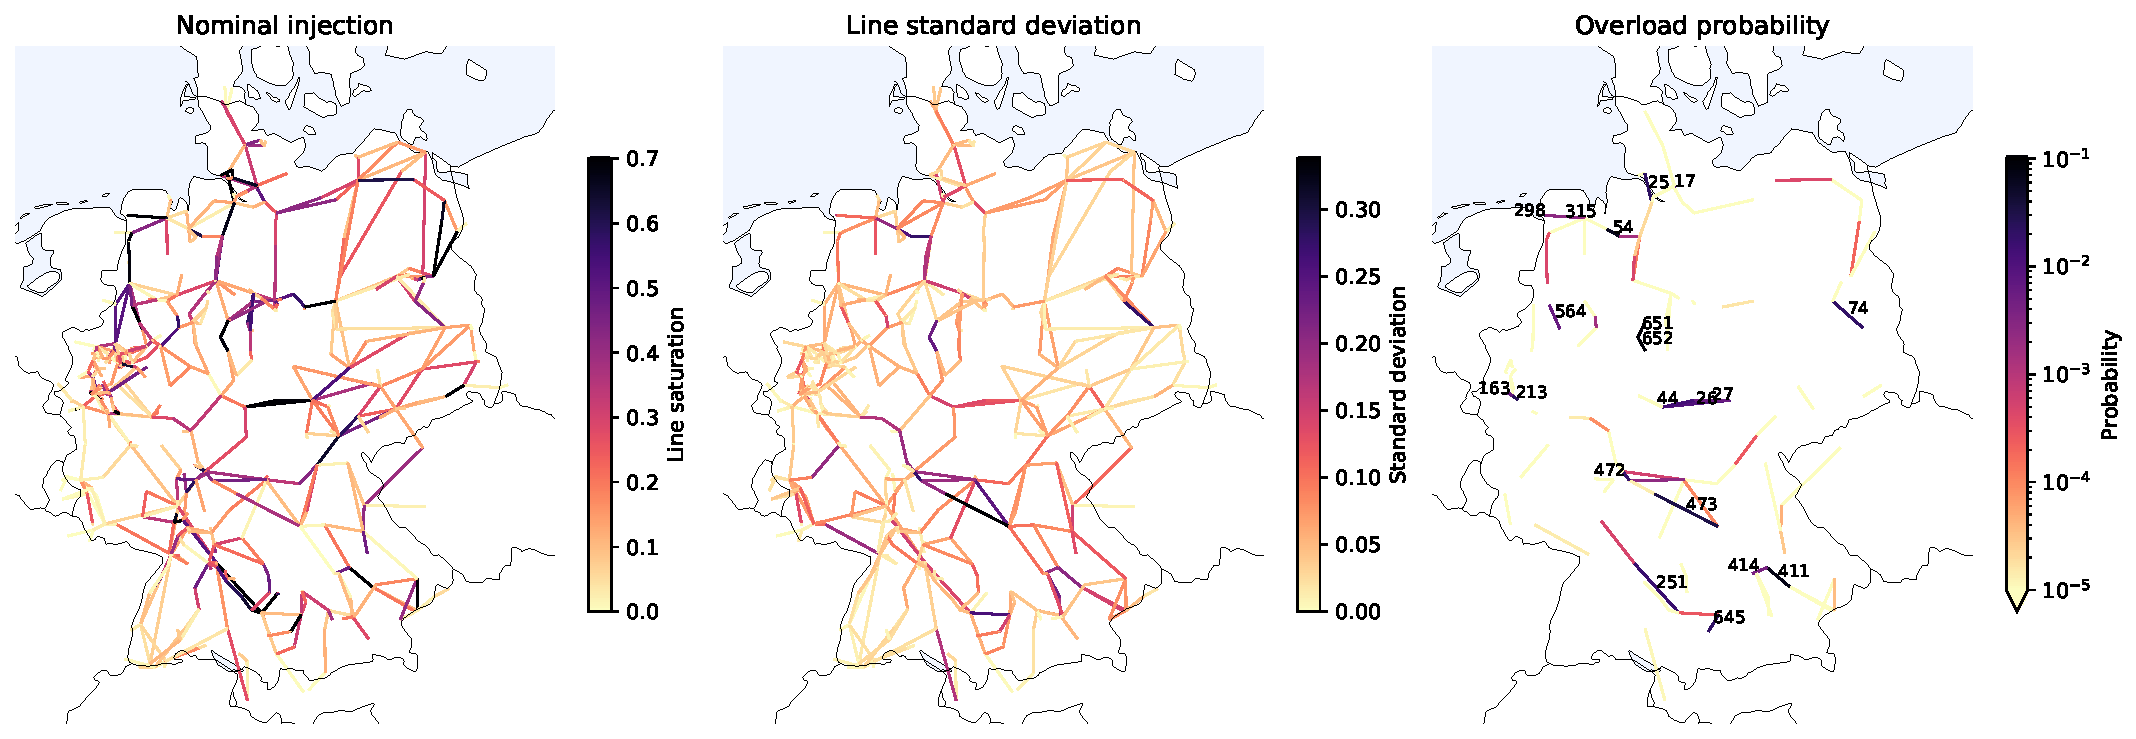
\includegraphics[width=\textwidth]{img/nomflow_stdev_trueoverloadprob_labeled.pdf}
    \caption{Visualisation of $\bm{\mu}_{\mathbf{f}}$, $\bm{\Sigma}_{\mathbf{f}}$ and $(\PROB\left[|\mel{f}_l| \geq 1 \right])_{l \in \range{m}}$ at 1 January, 11:00. The 20 most vulnerable lines are labelled.}
    \label{fig:nomflow_stdev_overload}
\end{figure}

\section{Most likely injection}
In addition to the failure probability, we compute the most likely injection to cause that failure using Theorem~\ref{thm:mostlikelyinjection}. The reader is invited to examine these injections themselves using Interactive~Figure~\ref{ifig:master}. The most likely fluctuation of three lines is given in Figure~\ref{fig:MLfluctuation1}. As expected, we find that vulnerable lines (most likely) fail due to small fluctuations in the injection, while robust lines only fail because of extreme, highly unrealistic fluctuations. 

\begin{figure}[ht]
\begin{subfigure}{\textwidth}
    \centering
    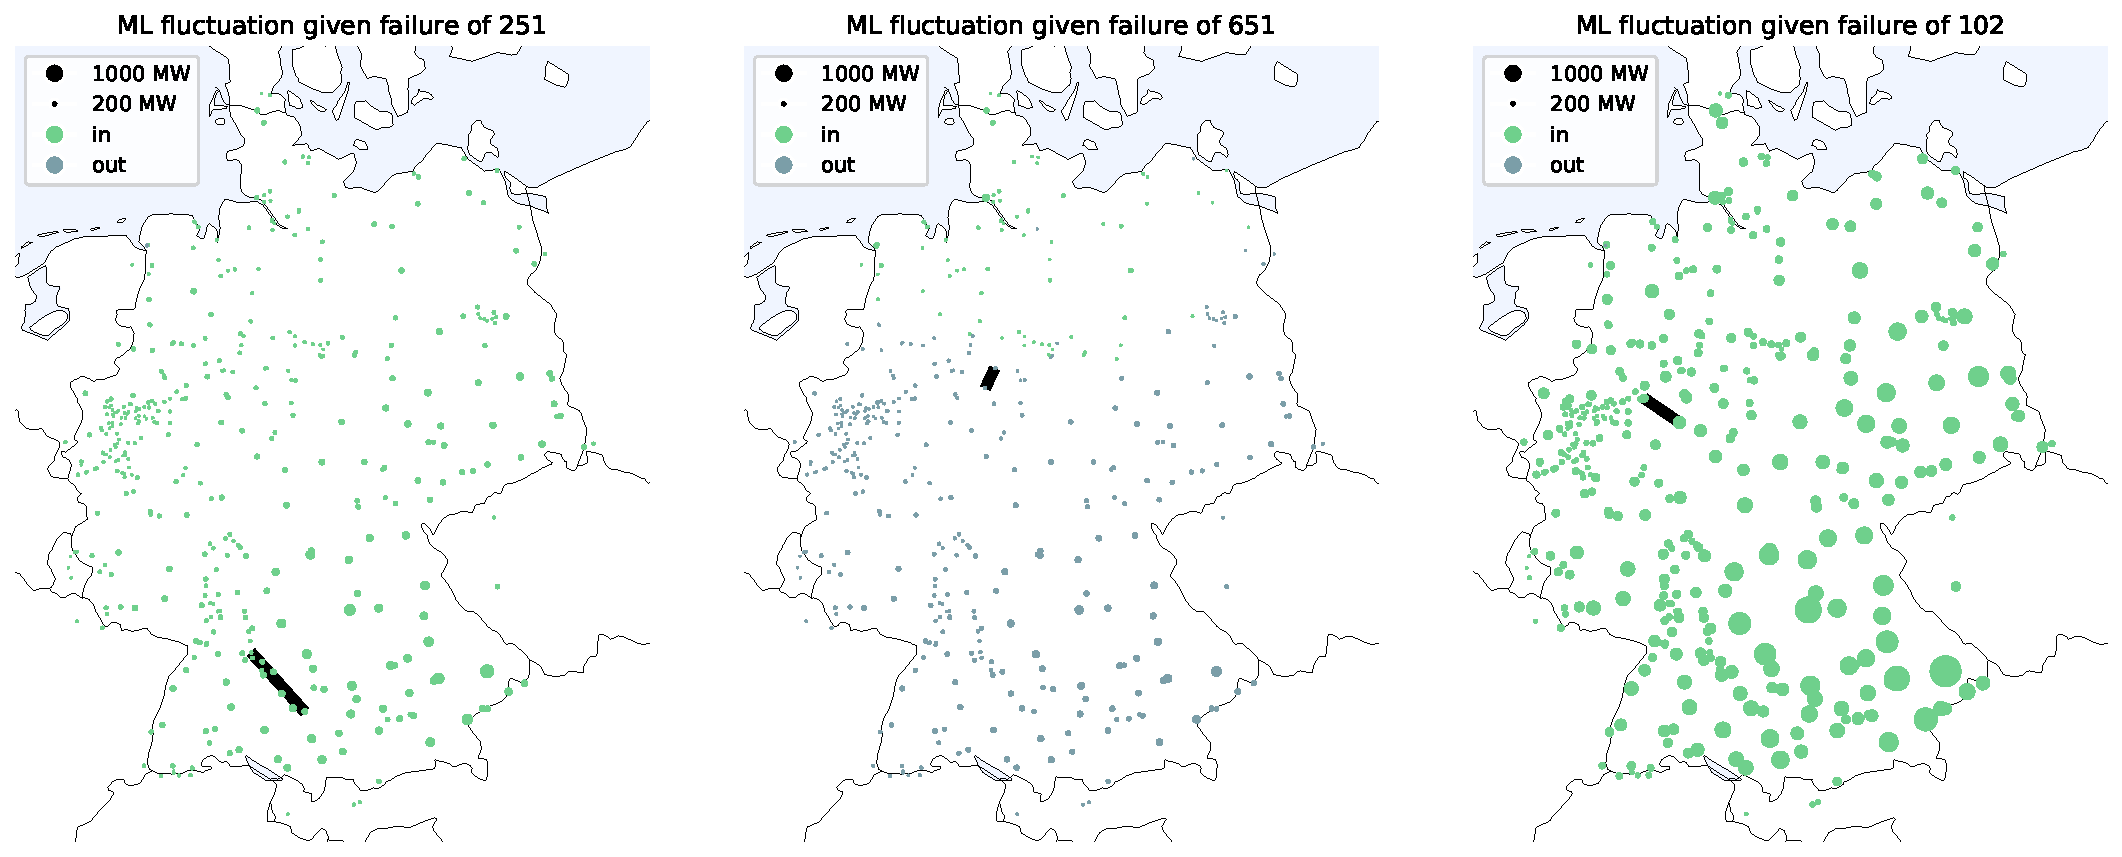
\includegraphics[width=\textwidth]{img/ML_fluctuation_with_bus_cov.pdf}
    \caption{Taking bus covariances into account.}\label{fig:MLfluctuation1}
\end{subfigure}
\begin{subfigure}{\textwidth}
    \centering
    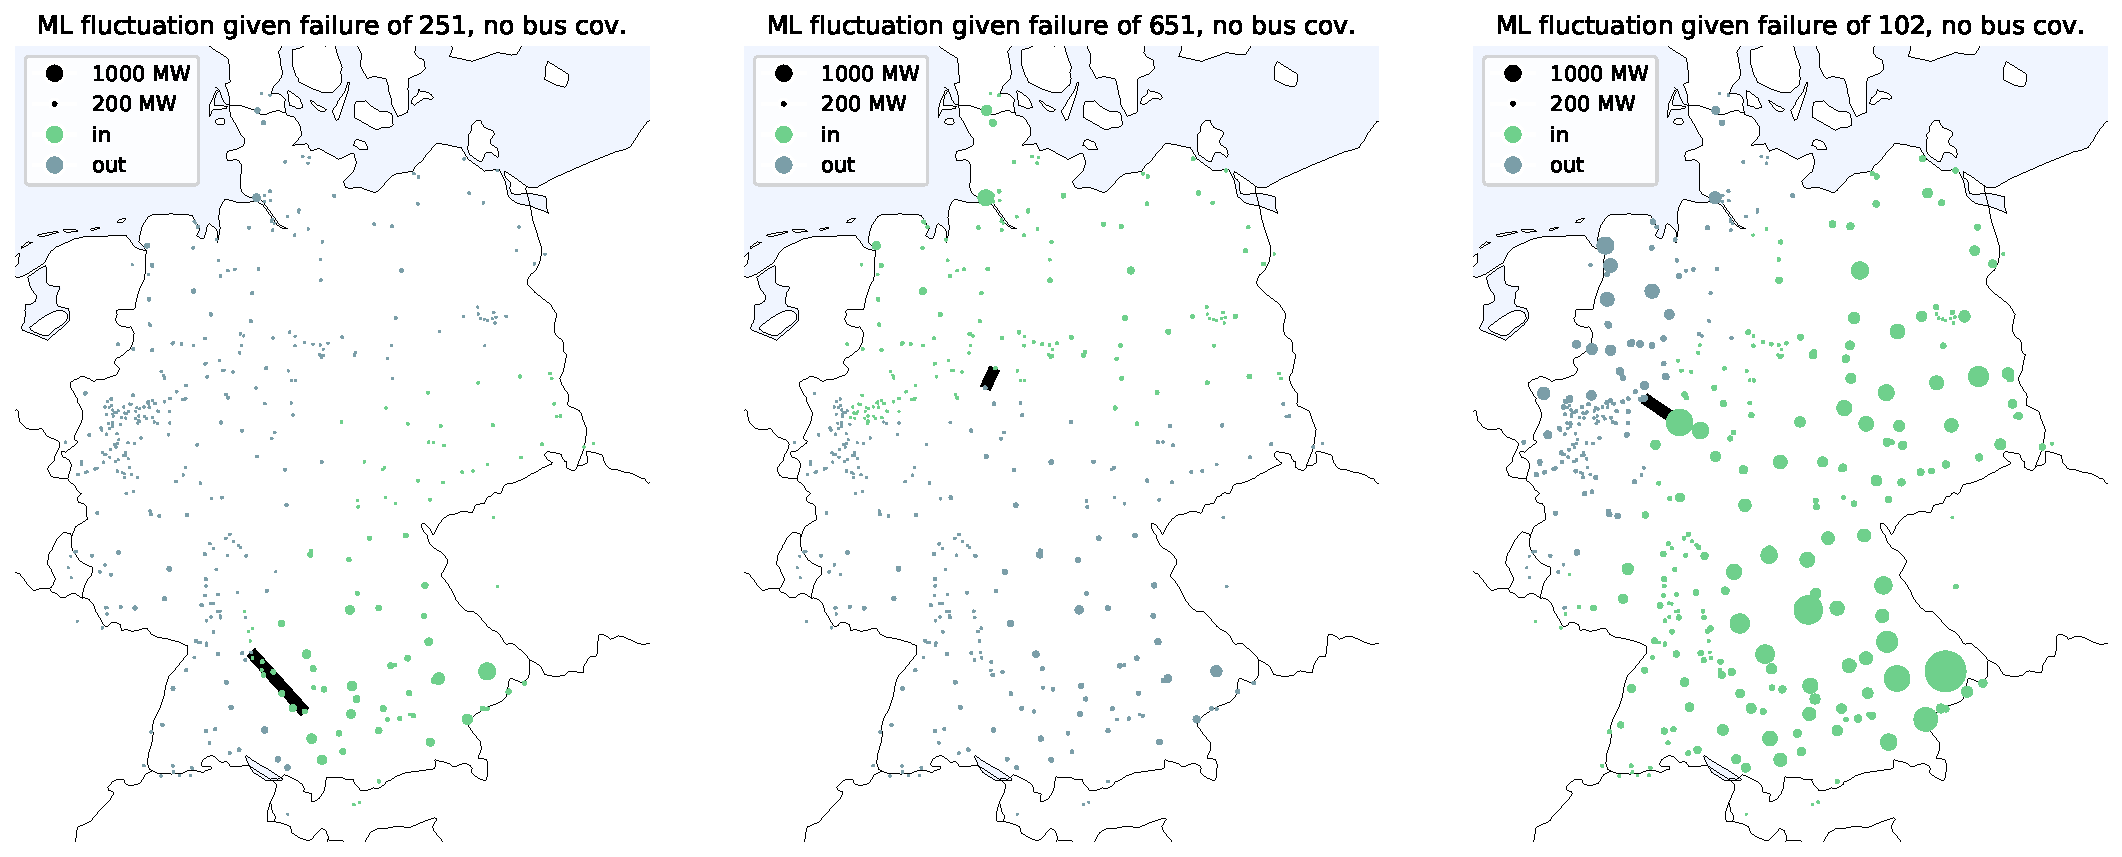
\includegraphics[width=\textwidth]{img/ML_fluctuation_without_bus_cov.pdf}
    \caption{Using only bus variances, with no covariance.}\label{fig:MLfluctuation2}
\end{subfigure}
    \caption{The most likely fluctuation given the failure of lines 251 (1.60\% overload probability), 651 (9.56\%) and 102 ($< 10^{-15}$). By including bus covariances (top), we find the most likely fluctuation to be more spread out. Zero-sum correction (distributive slack) is not applied.}\label{fig:MLfluctuation}
\end{figure}

\subsection{Geographic distribution of fluctuations}
In general, the most likely fluctuation is not concentrated at the two endpoints of the line, but rather, it consist of small, grid-wide fluctuations. This is due to high bus covariances, but also due to power flow physics. To examine the contribution of bus covariances, we also compute the most likely injection using only the diagonal of bus variances, see Figure~\ref{fig:MLfluctuation2}. For these three lines, we find that the fluctuations are indeed more evenly distributed when bus covariances are taken in account. 

To study this hypothesis more objectively, we need a measure of how `spread out' the fluctuation is. One possibility is to use the \emph{standard deviation} of the 489 entries of a fluctuation: when a fluctuation is more evenly distributed (geographically), we expect the standard deviation of individual fluctuations to be lower. When computing these values for the 50 most vulnerable lines, we find no significant result: the average of the 50 standard deviations in fluctuations is $22.0\,\si{MW}$ (SD $6.5\,\si{MW}$) for correlated buses and $22.6\,\si{MW}$ (SD $9.5\,\si{MW}$) for uncorrelated buses. Taking a lower number of lines does not improve the result. Curiously, when \emph{all} lines are considered (including the 584 lines with negligible overload probability\footnote{\ie less than $10^{-15}$, the numerical margin of error in our case}), the average standard deviation is actually \emph{higher} with correlated buses: $1245\,\si{MW}$ (SD $9244\,\si{MW}$) versus $418\,\si{MW}$ (SD $1036\,\si{MW}$) for uncorrelated buses. However, because we are mainly interested in the most vulnerable lines, we will leave this anomaly for what it is. Regarding the first 50 lines, it seems like a different approach is needed, and we are unable to confirm our hypothesis.

\subsection{Bus extensions}
Since we did not incorporate the \emph{installed stochastic capacity} in our model, it is possible that the predicted most likely injection dictates that some buses are generating more stochastic power than what is installed. To evaluate this problem, we retrieve the total amount of installed stochastic capacity for each bus from our dataset (taking the sum of solar and wind). For a given point in time, the generation values then tell us how much a bus can fluctuate upwards (more generation) and downwards. 

Given a most likely injection, we can compute whether the fluctuation at each bus is within the possible bounds, and if not, by how much the bounds must be extended for the most likely injection to be possible. In Table~\ref{tab:results}, the number of buses that needs to be extended is given, along with the total amount of extended capacity. For simplicity, we make no distinction between an extension upwards or downwards. An extension upwards means that more solar panels or wind turbines would be needed for the injection to be possible.\footnote{This implies an inaccuracy in our dataset.} An extension downwards is harder to justify, but one could say that it means that the amount of stochastic generation \emph{before} the fluctuation must have been higher, replacing non-stochastic generation at that node.

For the most vulnerable lines, we find that the \emph{number} of extended buses can be quite high, but the total amount of addition capacity is low, in general. For reference, buses in the network have an average installed capacity of $76\,\si{\mega\watt}$ (solar); $82\,\si{\mega\watt}$ (wind). 

\towrite{twee problemen: geen distr. slack meegenomen, geen onderscheid meer tussen zon en wind}

\towrite{het geeft vooral een mankement van het model aan: de grenzen zouden meegenomen moeten worden in de most likely injection}

\subsection{Cascades}
Using the most likely injection, we simulate the resulting cascade. The results for all lines are given in Interactive~Figure~\ref{ifig:master}. The number of lines that either failed jointly with the initial failure, or failed during the subsequent cascade, is also given in Table~\ref{tab:results}. This extends the result of \cite{Nesti2018supplemental}, which only provides the failure probability. We find that among the 10 most vulnerable lines (at 11:00),
only the failures of lines 298, 25 and 645 result in a power island. We will discuss these lines in more detail in Section~\ref{sec:evolution}, but for now, we note that these failures quickly result a power island. (For 298 and 645, this happens the first stage.) At this point, our model becomes unreliable (see Section~\ref{sec:discussioncasc}).

\begin{figure}[ht]
\renewcommand\figurename{Interactive Figure}
\begin{subfigure}{\textwidth}
    \centering
    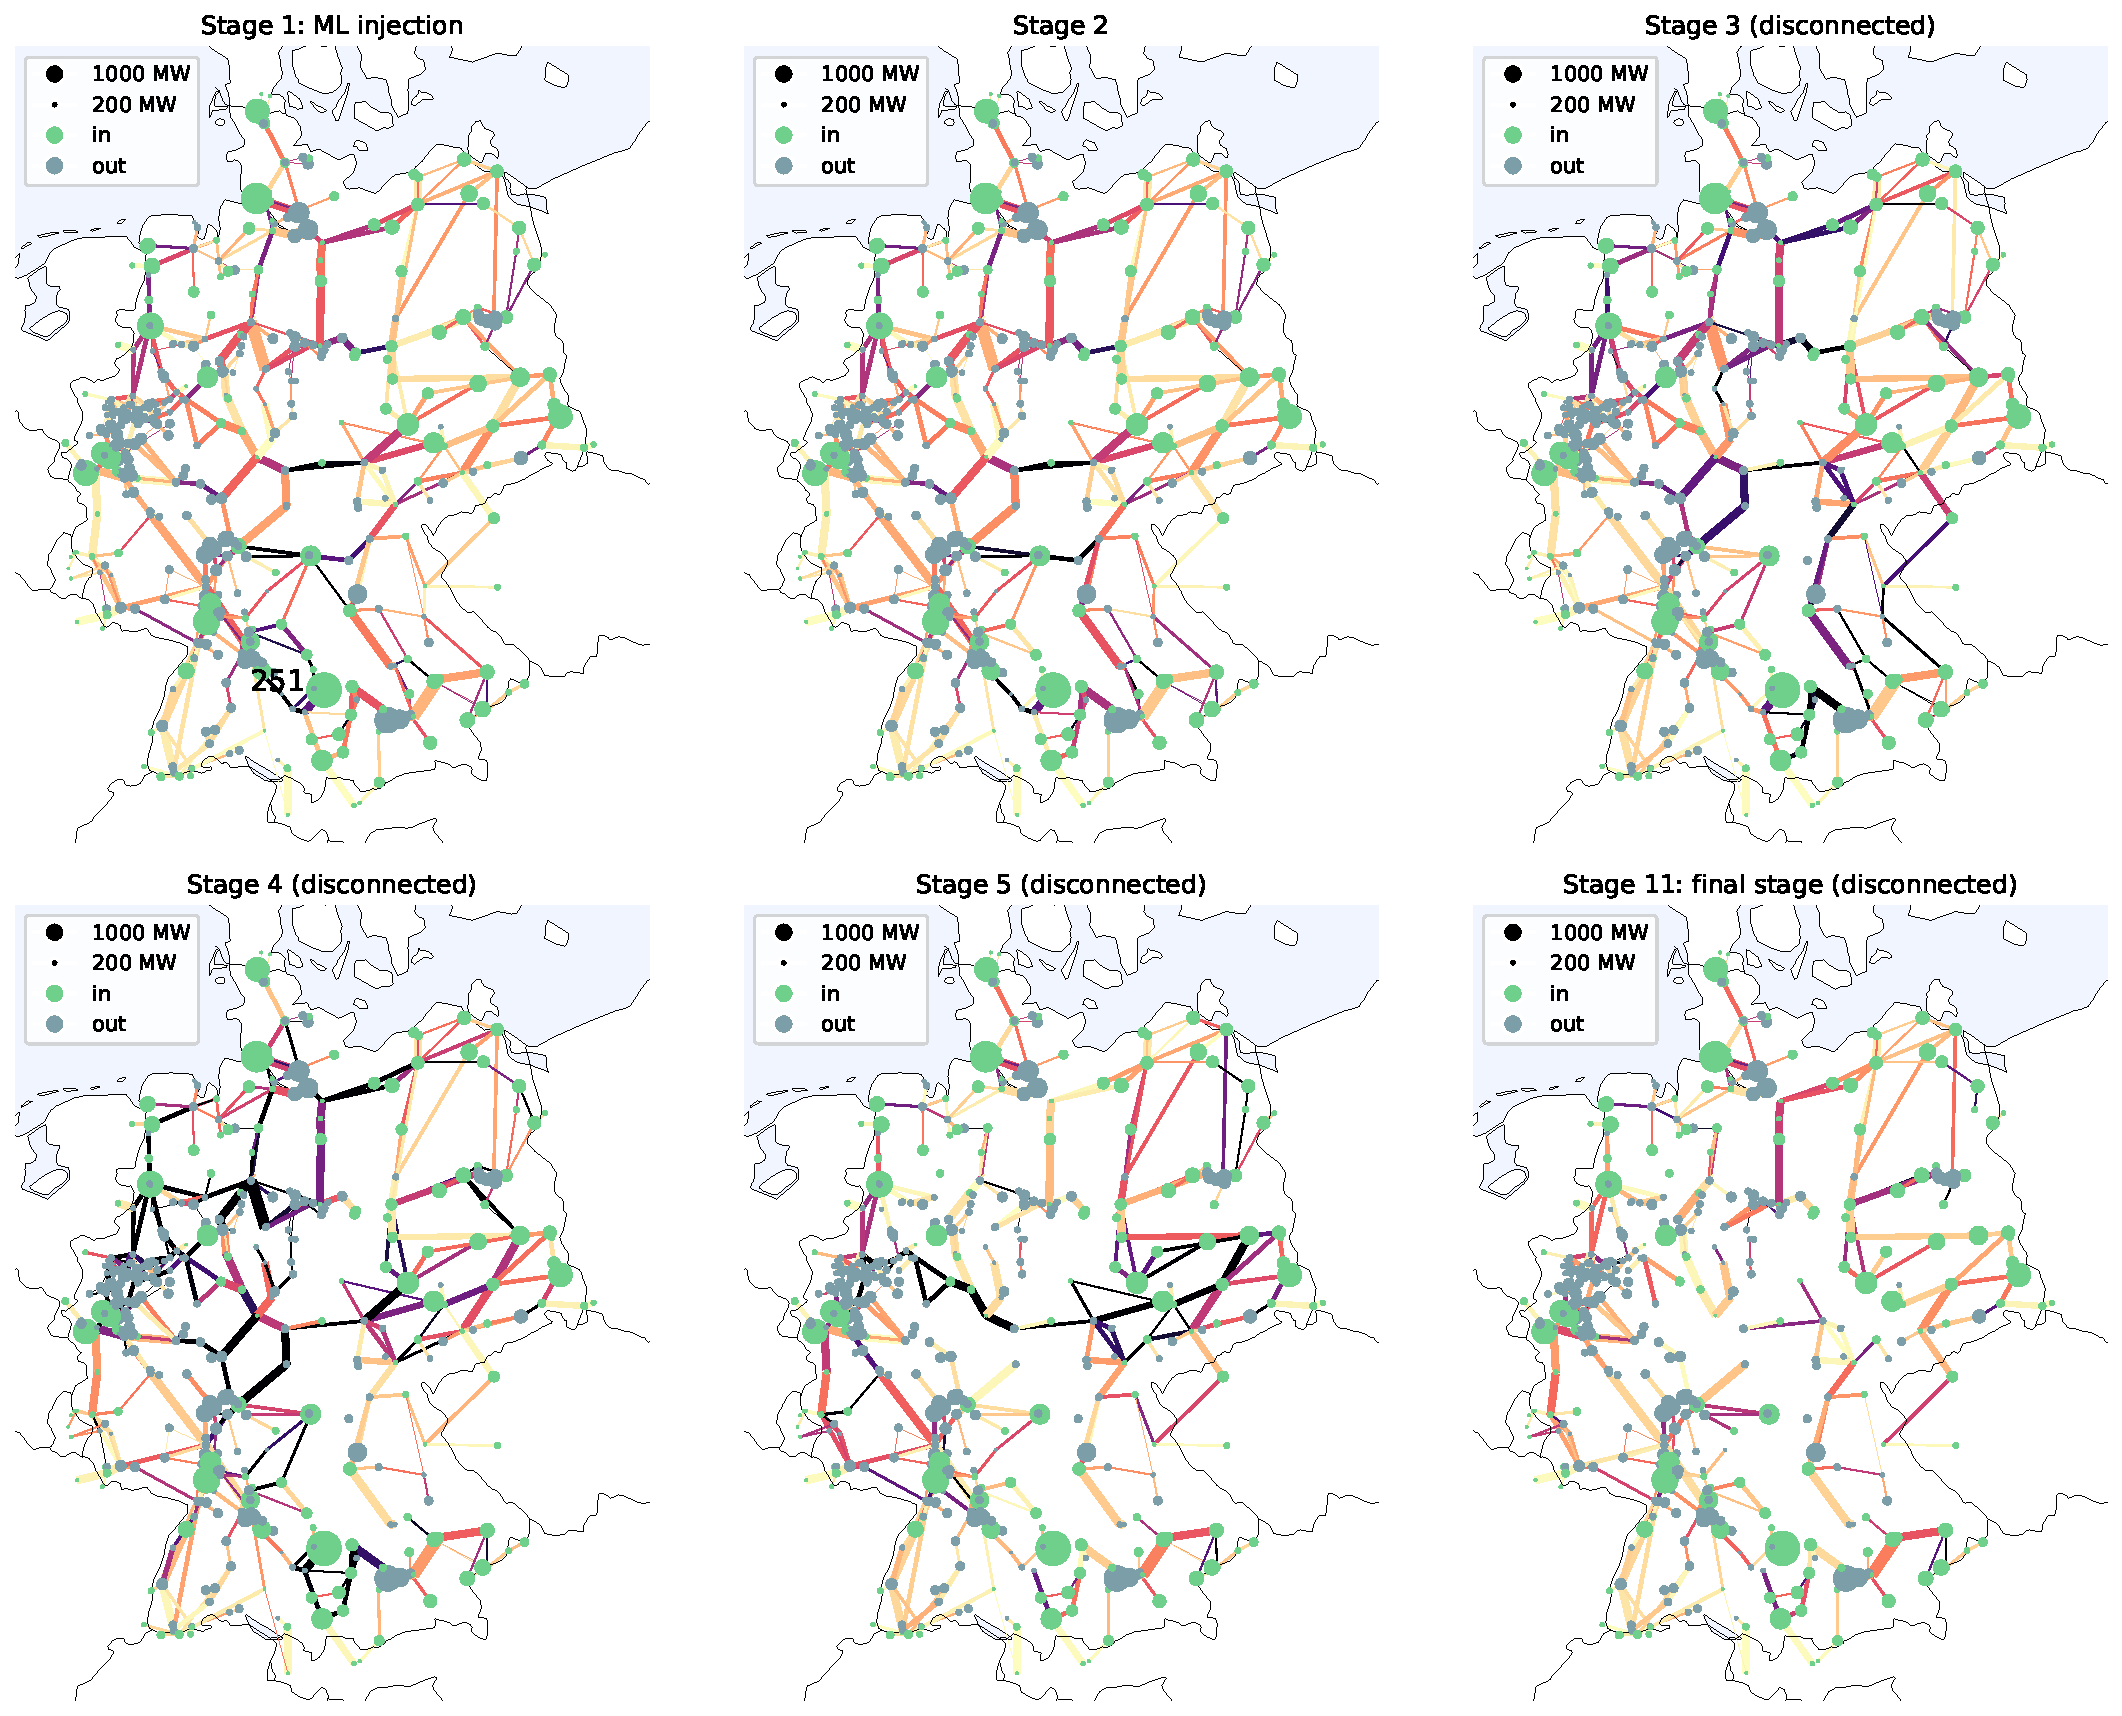
\includegraphics[width=\textwidth]{img/master_with_cov_251.pdf}
    \caption{Assumed failure of line 251.}\label{ifig:master251}
\end{subfigure}
%
\begin{subfigure}{\textwidth}
    \centering
    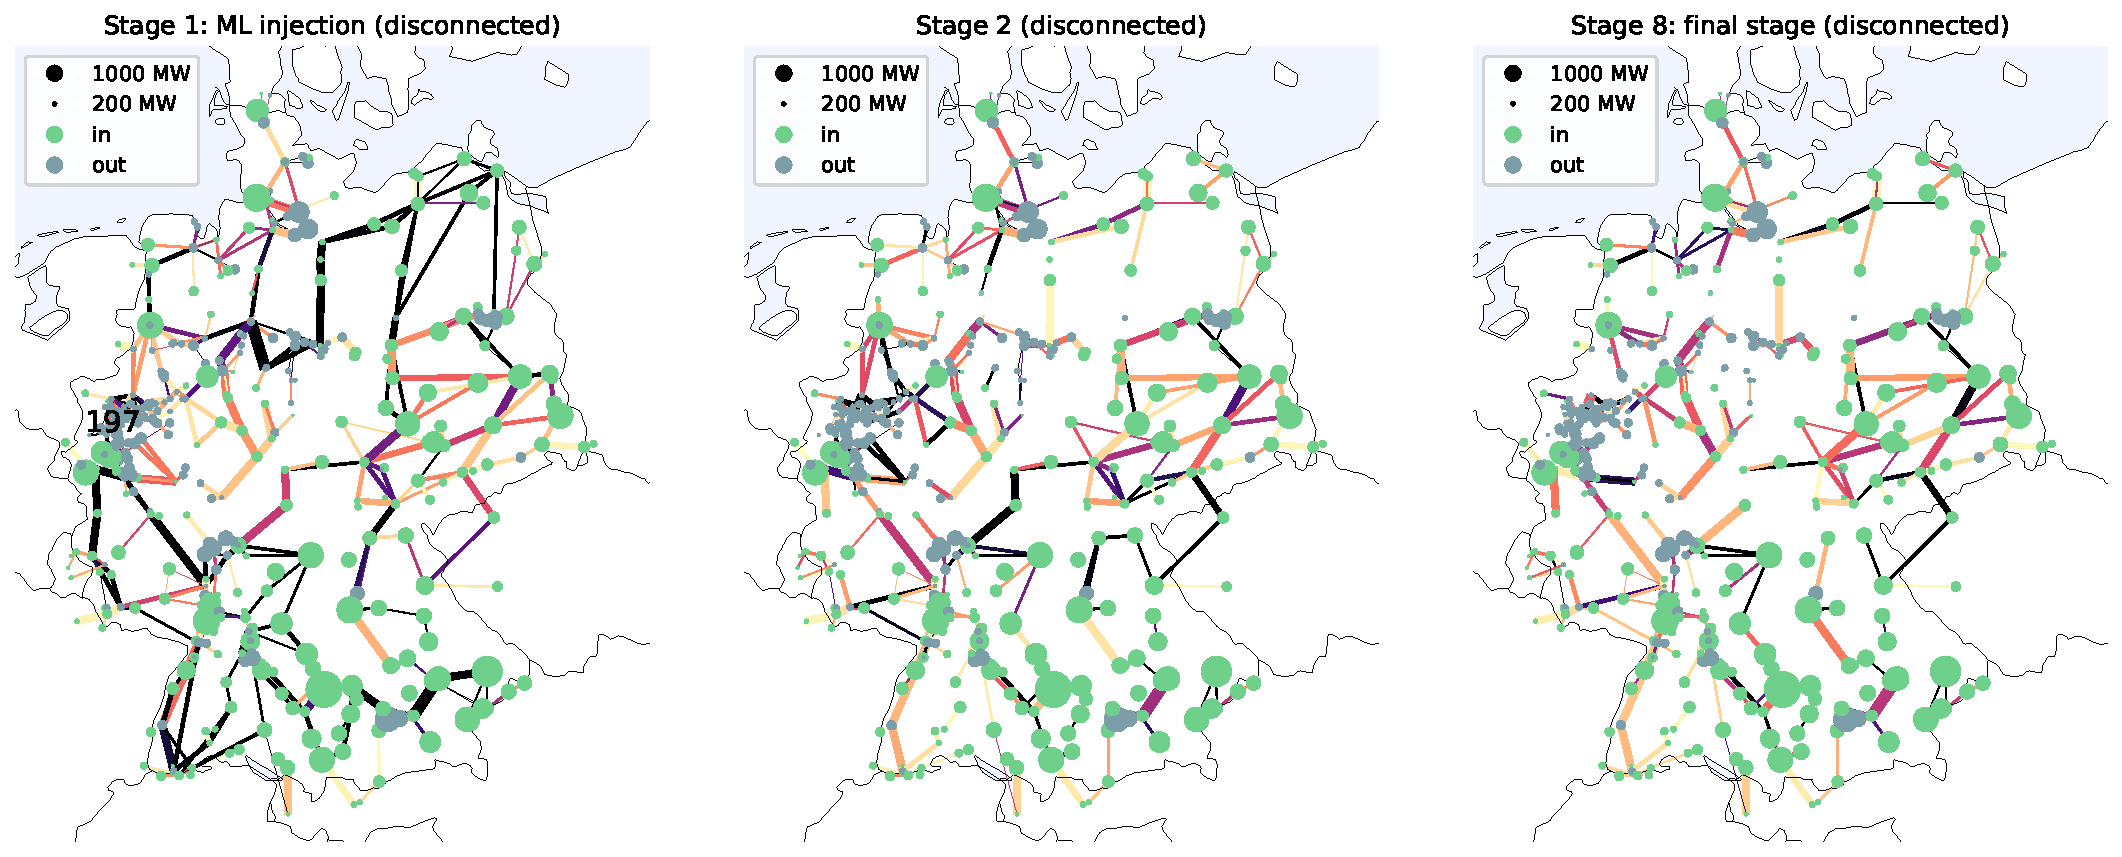
\includegraphics[width=\textwidth]{img/master_with_cov_197.pdf}
    \caption{Assumed failure of line 197.}\label{ifig:master197}
\end{subfigure}
%
    \caption{Simulated cascade stages after one assumed emergent failure. Node sizes represent the most likely injection. Long cascade sequences are truncated.
\vspace{.5em}
\newline
\emph{This figure is \textbf{interactive}: to view animated cascade simulations for all lines of the network, visit \href{https://fonsp.com/grid}{\texttt{fonsp.com/grid}}.}
}\label{ifig:master}
\end{figure}
\begin{figure}[ht]
\renewcommand\figurename{Interactive Figure}
\ContinuedFloat
\begin{subfigure}{\textwidth}
    \centering
    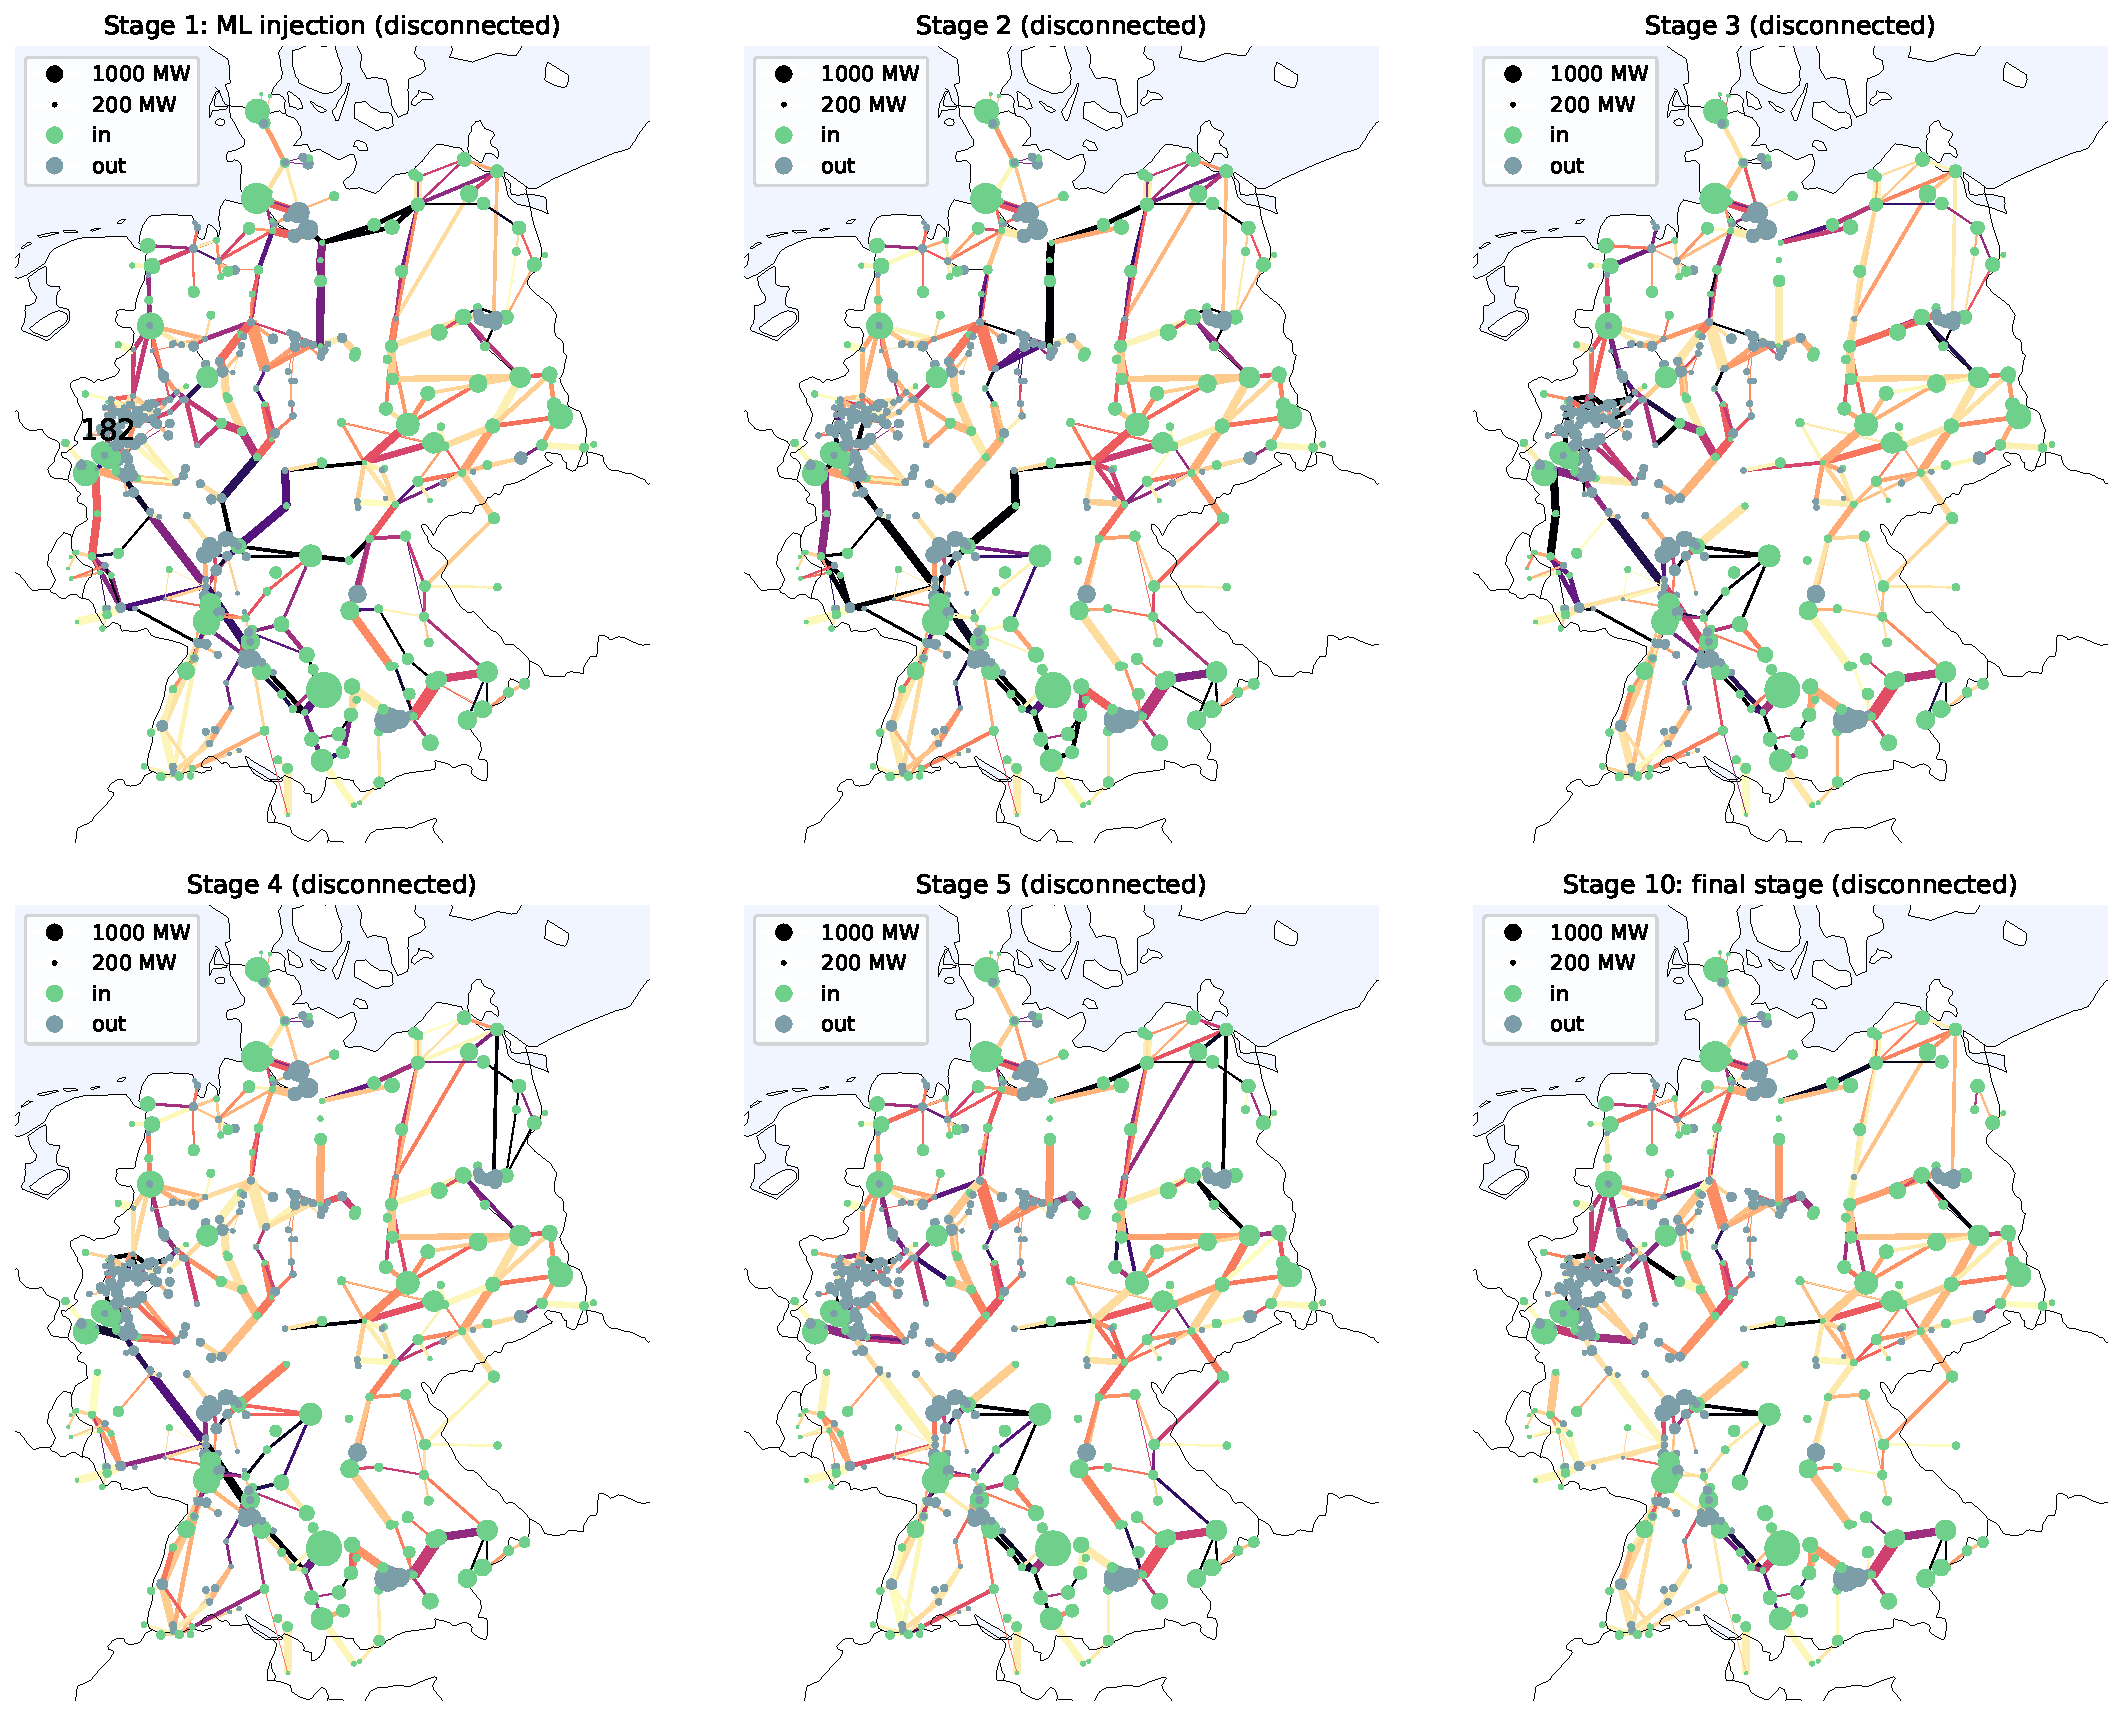
\includegraphics[width=\textwidth]{img/master_with_cov_182.pdf}
    \caption{Assumed failure of line 182.}\label{ifig:master182}
\end{subfigure}
%
    \caption{(continued).}\label{ifig:master}
\end{figure}

\subsubsection{Using the most likely injection}
\towrite{hoe zijn de resultaten anders wanneer we niet de mli nemen?}


\subsection{Evolution of line vulnerabilities}\label{sec:evolution}
Of course, the method above can be applied to any nominal injection, not just the injection at 1 January, 11:00. By applying the method to every hour of the first day, we find 24 different rankings, one of which is given in Table~\ref{tab:results}. This allows us to not only identify lines that are vulnerable at a given point in time, but to find lines that are a \emph{consistent vulnerability}, based on the general use of the transmission network.

Instead of providing 23 additional tables, we have summarised the results of a full day in Figure~\ref{fig:evolution_vulnerabilities}. Here, we see that some lines (like 337) are only vulnerable at one point during the day, while others (298 and 54) have a consistently high overload probability. There is a clear distinction between daytime and night-time, since the time of day determines which covariance matrix is used in the calculation. In fact, this highlights how a change in covariance influences results: some lines are only vulnerable because of the covariances brought upon by solar generation, while others are relatively unaffected.

A most striking result is that the overload probabilities of 25 and 298 are perfectly \emph{constant} for sustained periods, and both are likely to cause a cascade, resulting in an average of 108 and 76 failures, respectively. When examining these two lines in more detail, we find that both are \emph{branches out of the network towards coastal cities of the North Sea}, with high-capacity offshore wind generation. These generators were operating at full capacity during the studied day,\footnote{according to our dataset} which would cause a constant\footnote{except for the local energy usage, which is relatively small} power injection. Because the lines are \emph{branches} out of the larger graph, the flow through the line is exactly equal to the power injection at its end, and therefore constant.

Regarding the subsequent cascades of these two lines, it seems like our model falls short of giving an accurate redistribution of flow, due to the singularity caused by their removal. (No flow redistribution exists that would not change the injection.) 

\begin{figure}[ht]
\begin{subfigure}{\textwidth}
    \centering
    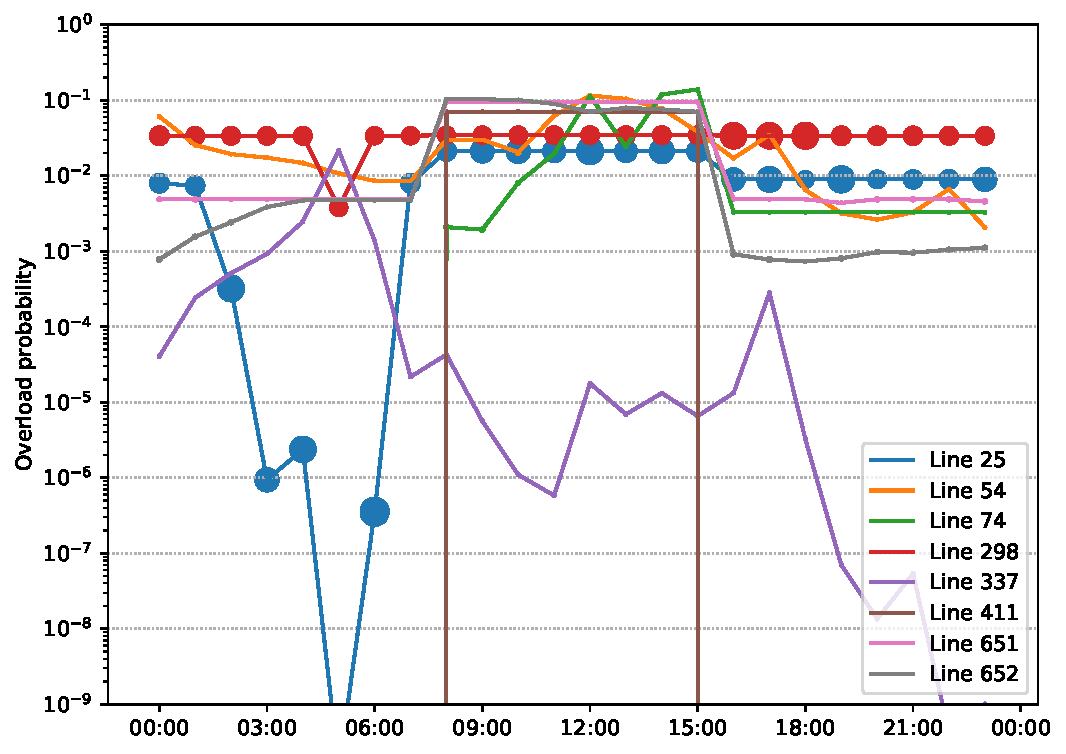
\includegraphics[width=\textwidth]{img/evolution_overload_probs_3.pdf}
    \caption{All lines that are, at any time during the day, among the 3 most vulnerable lines.}\label{fig:evolution_vulnerabilities_3}
\end{subfigure}
\begin{subfigure}{\textwidth}
    \centering
    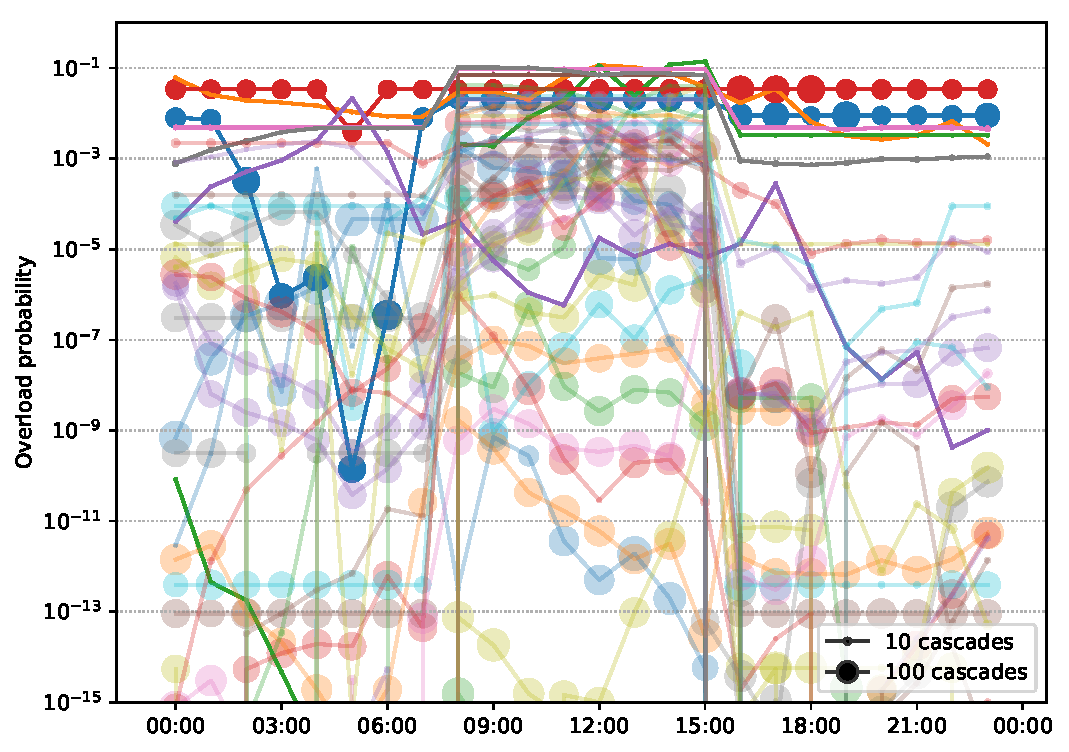
\includegraphics[width=\textwidth]{img/evolution_overload_probs_3_20.pdf}
    \caption{All lines that are, at any time during the day, among the 20 most vulnerable lines.}\label{fig:evolution_vulnerabilities_3_20}
\end{subfigure}
    \caption{\label{fig:evolution_vulnerabilities}Evolution of absolute failure probabilities during 1 January 2011. Dot sizes represent final number of lost lines after the most probable cascade.}
\end{figure}

\begin{figure}[ht]
    \centering
    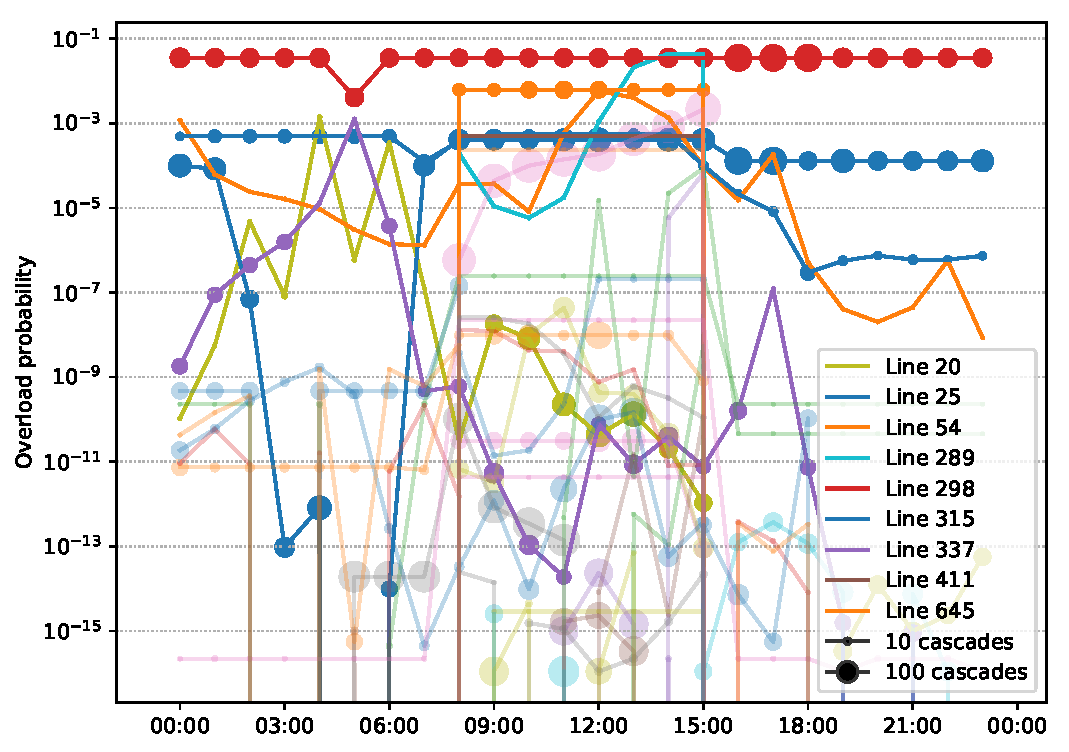
\includegraphics[width=\textwidth]{img/evolution_overload_probs_3_20_IID.pdf}
    \caption{For reference, the same as Figure~\ref{fig:evolution_vulnerabilities_3_20}, but computed using \emph{uncorrelated} injections.}\label{fig:evolution_vulnerabilities_3_20_IID}
\end{figure}


\subsection{Lines vulnerable to cascades}
\towrite{}


\begin{table}
\begin{tabular}{lll}
\toprule
$l$ & $\PROB \left[ |\mel{f}_l| \geq 1 \right]$ & $\mel{I}_l$ \\
\midrule
361 & 3.45\hphantom{0}\% &  1.65 \\
516 & 2.91\hphantom{0}\% &  1.79 \\
586 & 2.75\hphantom{0}\% &  1.84 \\
587 & 2.73\hphantom{0}\% &  1.85 \\
803 & 2.02\hphantom{0}\% &  2.10 \\
670 & 1.21\hphantom{0}\% &  2.54 \\
19  & 1.13\hphantom{0}\% &  2.60 \\
302 & 1.08\hphantom{0}\% &  2.64 \\
48  & 1.03\hphantom{0}\% &  2.68 \\
554 & 0.974\% &  2.73 \\
\midrule
488 & 0.971\% &  2.73 \\
809 & 0.824\% &  2.88 \\
28  & 0.748\% &  2.96 \\
810 & 0.728\% &  2.98 \\
29  & 0.396\% &  3.53 \\
27  & 0.355\% &  3.62 \\
389 & 0.247\% &  3.95 \\
390 & 0.245\% &  3.96 \\
486 & 0.235\% &  4.00 \\
249 & 0.056\% &  5.30 \\
\bottomrule
\end{tabular}

\caption{TODO}
\label{tab:top20old}
\end{table}

\begin{table}
\vspace{-1.5cm}
\centerline{
\begin{tabular}{lllrrllc}
\toprule
$l$ & $\PROB \left[ |\mel{f}_l| \geq 1 \right]$ & \multicolumn{1}{p{3em}}{mean $\pm$SD} & \multicolumn{1}{p{5em}}{\centering total {fluctuation}} & \multicolumn{2}{p{7em}}{extended buses (add. capacity)} & \multicolumn{1}{c}{cascade} & \multicolumn{1}{p{3em}}{\centering power \\ island?}\\
\midrule
\textbf{651} & \textbf{ 9.55\hphantom{0}\%} &  0.70$\pm$0.23 &       3.8 GW &      43 & (62 MW) & \multicolumn{1}{p{12em}}{                                              1 } &                 no \\
\textbf{652} & \textbf{ 8.95\hphantom{0}\%} &  0.68$\pm$0.24 &       3.9 GW &      46 & (82 MW) & \multicolumn{1}{p{12em}}{                                            (2) } &                yes \\
\textbf{411} & \textbf{ 7.06\hphantom{0}\%} &  0.70$\pm$0.20 &       5.0 GW &       6 & (12 MW) & \multicolumn{1}{p{12em}}{                                              1 } &                 no \\
\textbf{54 } & \textbf{ 6.21\hphantom{0}\%} &  0.61$\pm$0.25 &       2.5 GW &        3 & (1 MW) & \multicolumn{1}{p{12em}}{                                              1 } &                 no \\
\textbf{298} & \textbf{ 3.45\hphantom{0}\%} &  0.70$\pm$0.17 &       1.1 GW &        3 & (0 MW) & \multicolumn{1}{p{12em}}{                          (1 >> 3 >> ... >> 65) } &                yes \\
\textbf{473} & \textbf{ 3.13\hphantom{0}\%} &  0.37$\pm$0.34 &       7.1 GW &      10 & (52 MW) & \multicolumn{1}{p{12em}}{                                              1 } &                 no \\
\textbf{213} & \textbf{ 2.37\hphantom{0}\%} &  0.70$\pm$0.15 &       6.9 GW &    103 & (569 MW) & \multicolumn{1}{p{12em}}{                               2 >> 3 >> 4 >> 5 } &                 no \\
\textbf{25 } & \textbf{ 2.11\hphantom{0}\%} &  0.70$\pm$0.15 &       2.1 GW &        0 & (0 MW) & \multicolumn{1}{p{12em}}{              2 >> 4 >> (5 >> 50 >> ... >> 102) } &                yes \\
\textbf{645} & \textbf{ 2.02\hphantom{0}\%} &  0.70$\pm$0.15 &       4.4 GW &      15 & (70 MW) & \multicolumn{1}{p{12em}}{                          (1 >> 5 >> ... >> 53) } &                yes \\
\textbf{74 } & \textbf{ 1.96\hphantom{0}\%} &  0.43$\pm$0.28 &       6.5 GW &      12 & (52 MW) & \multicolumn{1}{p{12em}}{                                              1 } &                 no \\
\textbf{472} & \textbf{ 1.76\hphantom{0}\%} &  0.43$\pm$0.27 &       8.3 GW &      11 & (84 MW) & \multicolumn{1}{p{12em}}{                                              2 } &                 no \\
\textbf{251} & \textbf{ 1.60\hphantom{0}\%} &  0.70$\pm$0.14 &       7.6 GW &     11 & (111 MW) & \multicolumn{1}{p{12em}}{             2 >> 5 >> (10 >> 19 >> ... >> 177) } &                yes \\
\textbf{44 } & \textbf{ 1.31\hphantom{0}\%} &  0.70$\pm$0.14 &       9.1 GW &       9 & (33 MW) & \multicolumn{1}{p{12em}}{                                         1 >> 2 } &                 no \\
\textbf{26 } & \textbf{ 0.980\%} &  0.70$\pm$0.13 &       9.4 GW &       9 & (46 MW) & \multicolumn{1}{p{12em}}{              1 >> 3 >> (8 >> 23 >> ... >> 117) } &                yes \\
\textbf{17 } & \textbf{ 0.871\%} &  0.70$\pm$0.13 &       6.5 GW &     70 & (324 MW) & \multicolumn{1}{p{12em}}{                                              3 } &                 no \\
\textbf{163} & \textbf{ 0.645\%} &  0.70$\pm$0.12 &       9.1 GW &   143 & (1137 MW) & \multicolumn{1}{p{12em}}{                                    2 >> 3 >> 4 } &                 no \\
\textbf{564} & \textbf{ 0.585\%} &  0.70$\pm$0.12 &       5.9 GW &        1 & (2 MW) & \multicolumn{1}{p{12em}}{                                              2 } &                 no \\
\textbf{27 } & \textbf{ 0.542\%} &  0.69$\pm$0.12 &      10.1 GW &      10 & (69 MW) & \multicolumn{1}{p{12em}}{                             2 >> 3 >> (5 >> 8) } &                yes \\
\textbf{414} & \textbf{ 0.406\%} &  0.47$\pm$0.20 &       9.8 GW &     12 & (140 MW) & \multicolumn{1}{p{12em}}{                       2 >> 3 >> 4 >> (6 >> 10) } &                yes \\
\textbf{315} & \textbf{ 0.246\%} &  0.70$\pm$0.11 &       2.0 GW &        0 & (0 MW) & \multicolumn{1}{p{12em}}{                                 (2 >> 7 >> 13) } &                yes \\
\textbf{461} & \textbf{ 0.237\%} &  0.46$\pm$0.19 &      10.7 GW &     15 & (234 MW) & \multicolumn{1}{p{12em}}{                                    2 >> 4 >> 5 } &                 no \\
\textbf{627} & \textbf{ 0.160\%} &  0.57$\pm$0.15 &       8.3 GW &     23 & (169 MW) & \multicolumn{1}{p{12em}}{                                              2 } &                 no \\
\textbf{531} & \textbf{ 0.151\%} &  0.18$\pm$0.28 &       5.2 GW &      14 & (56 MW) & \multicolumn{1}{p{12em}}{                        (3 >> 11 >> ... >> 159) } &                yes \\
\textbf{534} & \textbf{ 0.113\%} &  0.63$\pm$0.12 &       4.3 GW &        2 & (8 MW) & \multicolumn{1}{p{12em}}{              3 >> 5 >> (8 >> 12 >> ... >> 184) } &                yes \\
\textbf{460} & \textbf{ 0.052\%} &  0.38$\pm$0.19 &      12.5 GW &     20 & (396 MW) & \multicolumn{1}{p{12em}}{                 3 >> 6 >> 7 >> 8 >> (11 >> 12) } &                yes \\
\textbf{257} & \textbf{ 0.048\%} &  0.51$\pm$0.15 &      10.3 GW &     21 & (417 MW) & \multicolumn{1}{p{12em}}{                            3 >> 6 >> (8 >> 11) } &                yes \\
\textbf{624} & \textbf{ 0.047\%} &  0.42$\pm$0.17 &       5.5 GW &      13 & (53 MW) & \multicolumn{1}{p{12em}}{        3 >> 6 >> 9 >> 15 >> (21>>...>>137) } &                yes \\
\textbf{561} & \textbf{ 0.045\%} &  0.68$\pm$0.10 &       4.7 GW &        1 & (2 MW) & \multicolumn{1}{p{12em}}{             3 >> 9 >> 16 >> (21 >> ... >> 200) } &                yes \\
\textbf{569} & \textbf{ 0.042\%} &  0.61$\pm$0.12 &       8.4 GW &      19 & (87 MW) & \multicolumn{1}{p{12em}}{                  1 >> (4 >> 179 >> ... >> 219) } &                yes \\
\textbf{563} & \textbf{ 0.034\%} &  0.69$\pm$0.09 &       4.5 GW &        2 & (8 MW) & \multicolumn{1}{p{12em}}{             3 >> 8 >> (16 >> 52 >> ... >> 151) } &                yes \\
%\textbf{422} & \textbf{ 0.027\%} &  0.10$\pm$0.26 &      12.8 GW &   196 & (2309 MW) & \multicolumn{1}{p{12em}}{                                    3 >> 4 >> 5 } &                 no \\
%\textbf{387} & \textbf{ 0.026\%} &  0.64$\pm$0.10 &       9.4 GW &   151 & (1548 MW) & \multicolumn{1}{p{12em}}{      4 >> 8 >> 17 >> (47 >> 173 >> ... >> 209) } &                yes \\
%\textbf{185} & \textbf{ 0.019\%} &  0.70$\pm$0.08 &       7.3 GW &     76 & (496 MW) & \multicolumn{1}{p{12em}}{              3 >> 7 >> (8 >> 15 >> ... >> 144) } &                yes \\
%\textbf{333} & \textbf{ 0.014\%} &  0.39$\pm$0.17 &       5.5 GW &       6 & (38 MW) & \multicolumn{1}{p{12em}}{            4 >> 10 >> (17 >> 23 >> ... >> 126) } &                yes \\
%\textbf{458} & \textbf{ 0.010\%} &  0.10$\pm$0.24 &      14.3 GW &     28 & (601 MW) & \multicolumn{1}{p{12em}}{                          4 >> (10 >> 12 >> 13) } &                yes \\
%\textbf{535} & \textbf{ 0.008\%} &  0.35$\pm$0.17 &      16.5 GW &     28 & (530 MW) & \multicolumn{1}{p{12em}}{                  4 >> (11 >> 15 >> ... >> 152) } &                yes \\
%\textbf{393} & \textbf{ 0.004\%} &  0.41$\pm$0.15 &      11.3 GW &   195 & (2435 MW) & \multicolumn{1}{p{12em}}{                                         4 >> 6 } &                 no \\
%\textbf{386} & \textbf{ 0.003\%} &  0.70$\pm$0.08 &      12.4 GW &     23 & (474 MW) & \multicolumn{1}{p{12em}}{               3 >> 7 >> (12 >> 26 >> 28 >> 30) } &                yes \\
%\textbf{623} & \textbf{ 0.002\%} &  0.36$\pm$0.16 &       5.4 GW &       2 & (33 MW) & \multicolumn{1}{p{12em}}{             4 >> 9 >> (17 >> 65 >> ... >> 116) } &                yes \\
%\textbf{446} & \textbf{ 0.002\%} &  0.47$\pm$0.13 &      13.5 GW &   227 & (2998 MW) & \multicolumn{1}{p{12em}}{                                       (3 >> 5) } &                yes \\
\bottomrule
\end{tabular}

}
\vspace{1cm}
\caption{The 30 most vulnerable lines at 1 January, 11:00. For each line, we have the absolute overload probability and the mean and standard deviation of line saturation. For the most likely injection, the total change (fluctuation) in injection is given, and the number of buses for which renewable generation would need to be extended for the most likely injection to be possible. \protect\newline
The number of failed lines in each cascade stage is shown. Stages in parentheses correspond to a disconnected network. (The first number is greater than $1$ when there are \emph{joint failures}.) The final column states whether the last cascade stage is disconnected (\ie whether a power island emerged).
}
\label{tab:results}
\end{table}

\section{Discussion}
\subsection{Cascading failures}\label{sec:discussioncasc}
Following \cite{Nesti2018emergentfailures}, we compute the lines most vulnerable to emergent failures, and we give the absolute overload probability (first two columns of Table~\ref{tab:results}). We extend their result by also stating the (most likely) total fluctuation and the sequence of cascades. Additionally, we asses the final stage of the cascade (\ie the \emph{severity} of the emergent failure) using the final number of failed lines, and we determine whether a power island emerged in the process.

This allows us to make the important observation that most vulnerable lines do not result in a severe cascade of failures. This means that the network will remain operational after the emergent failure, and once the nefarious fluctuation has passed, the failed line can be operational again. For some vulnerable lines, our model does predict a significant amount of cascaded failures. However, when looking at these cases individually, we find that they are all lines that branch out of the network, quickly resulting in a power island. After the power island occurred, the simulated cascades are likely erroneous. We suspect that the emergent failure of these lines will indeed cause a power island to form, but that the remainder of the network will remain operational.

\subsection{Power islands}\label{sec:discussionpowerislands}
The Optimised method computes redistributed flows efficiently, and its derivation (Section \ref{sec:optimisedmethod}) provides us with a more intuitive understanding of flow redistribution. Examining results for individual lines (\eg see Interactive Figure \ref{ifig:master}) shows realistic results. Yet, as we the analyses of lines 25 and 298 demonstrate, the method is likely erroneous when the network becomes \emph{disconnected} after the line removal(s), \ie when a power island occurs.

In fact, in its original form \citep{Ronellenfitsch2017}, the optimised method is only defined when the network remains connected.
While this is a limitation of the Optimised method, it is, more generally, a limitation of using DC approximated power flow. In this approximation, we assume the network to be in a \emph{state of equilibrium}: generation matches load exactly. 

In our case, the use of a stochastic injection means that we generally do not have a zero-sum injection, contracting the assumption. This contradiction is usually justified using the concept of (distributive) slack: an overall increase or decrease in generation will occur (to compensate for the non-zero net injection), without changing the line flows.

Yet, when studying cascading failures, we are looking at a time frame much shorter than the time it takes to reach equilibrium. 
This shorter time scale generally requires an analysis of an entirely different nature: this is the study of \emph{transient stability}, which is far beyond the scope of this thesis. 

Overall, a better understanding of the physics that underlie line failures is required to study cascading failures, especially in cases where power islanding occurs. 

\subsection{Previous work \citep{Nesti2018emergentfailures}}\label{sec:discussionnesti}
This thesis was inspired by the model and case study of \cite{Nesti2018emergentfailures}. While many of the future research topics proposed by this article remain open, we have been able to independently verify their results. While our model is based on the original, there are some fundamental differences between the two. Therefore, the differences in our results provide valuable insight into the accuracy of either model. 

There are two important modifications that we chose to make to the original model. First of all, our model does not use ARMA forecasting, but a much simpler \emph{persistent forecast} as placeholder. For wind generation series, the resulting covariance matrices turn out to be very similar. We cannot comment on the similarity in solar covariances, as we were unable to reproduce these results.

A second difference is the use of a different method for computing the redistributed flow, which is based on \cite{Ronellenfitsch2017}. There is no clear practical benefit to using the Optimised method, except for computational cost. Still, our use of this method has led to the insight that a DC approximated model is not well-suited for disconnected networks, when a large power imbalance exists among connected islands. Although these problems can be justified using the notion of \emph{distributive slack} TODO

This Optimised method requires the network to be a \emph{digraph}, which does not allow for parallel lines to exist. For this reason, we have combined parallel lines in our network, taking their physical properties into account. Strangely, this increases the discrepancy between the line flows computed by the LPF, and those given by the OPF algorithm. This effect could be investigated further by studying smaller test networks.


\subsubsection{Evaluation of results}
We performed a careful analysis of the results that follow from the SciGRID application, identifying new problems in the model of \cite{Nesti2018emergentfailures}. For example, we find that for almost all lines, the most likely power injection requires an extension of stochastic capacity at multiple buses. For some lines, this extension is relatively small, and it does not invalidate the result. For other lines, a significant extension is needed. We suspect that the required extensions will be much greater when analysing a point in time when renewable generation is already high. A better understanding of the origin of our dataset is needed to evaluate the significance of this problem.

This problem could be addressed \emph{within the framework of our model} by imposing additional conditions on the most likely injection. In its current form, the problem of finding the most likely injection is an optimisation problem with \emph{linear boundary conditions} (as given in the proof of Theorem~\ref{thm:mostlikelyinjection}). Because the boundary conditions can be written as a \emph{half-plane in $\mathbb{R}^n$}, we were able to derive a closed form solution. We could include the upper and lower limits of stochastic generation as addition linear conditions, which will likely make a closed-form solution unobtainable. Instead, non-linear optimisation methods could be used to find the most likely injection, given these additional conditions.\footnote{In fact, if we use this more general method to find the most likely injection, we could enforce the power injection to have zero sum by imposing one additional linear condition: $\sigma (\mat{p}) = 0$. Although this would solve the problem of having a most likely injection with non-zero sum, there is no physical argument for this imposing this condition.} See \cite{Chertkov2011} for a study using this approach.

\subsection{Future}
There are many aspects of this analysis that could should be studied in more detail, some of which are mentioned throughout this chapter. Regarding our case study, the first shortcoming that could be addressed is the fact that we have only thoroughly looked at the data of January 1$^{st}$. Like \cite{Nesti2018emergentfailures}, most of our results are computed for the nominal injection at 11:00. Additionally, we have computed our main result for the remaining 23 hours of the day, which includes hours where the \emph{night} covariance matrix is used (see Figure~\ref{fig:evolution_vulnerabilities}). 
While we can directly compute results for the remaining days of January and the remaining months of 2011, we have not yet analysed these results.

While our dataset provides an interesting case study, it does have some limitations. First of all, the dataset does not consist of physical measurements: it is constructed by combining various data sources, most of which are in turn the obtained from modelling. Because of the various steps needed to construct a full dataset, it is hard to quantify the inaccuracy of our results. 

Crucially, our dataset does not allow us to \emph{verify our results}, since it is \emph{too coarse} to contain fluctuations, and it provides no historical data on line failures. High-resolution stochastic generation datasets do exist, possibly for all nodes of a realistic transmission network. However, to the best of our knowledge, no dataset exist that contains continuous measurements of line currents and overloads. 

Many smaller datasets exists that can be analysed using our methods. Most notably, the \emph{IEEE test networks} can be extended with fictional stochastic generation, as demonstrated by \cite{Nesti2018emergentfailures} and \cite{Chertkov2011}. These smaller networks would allow us to more easily inspect the behaviour of individual lines in the network. Another way to construct a smaller network could be to take a \emph{subsection} of the SciGRID network.

\towrite{

Verschillen:
- economie


Kritiek op nesti:

- ze nemen een contingency factor van 0.7 bij de OPF (arbitrair) maar voor de analyse van cascades niet. (toch?)

- non-zero injection problem


Of course, this has the same shortcoming as the model used by \cite{Nesti2018emergentfailures} (it ), but it 

Although these ARMA models are fairly involved, they do not actually provide an accurate forecast.TODOfootnote{\cite{Nesti2018emergentfailures} also express this fact in their article, and note that it is only the forecast \emph{error} that is relevant in our analysis.} Using ARMA models seems unnecessarily complicated
}



\clearpage
\end{document}